\documentclass[a4paper]{report}

\usepackage[french]{babel}
\usepackage{amsfonts, amssymb, amsthm, amsmath, mathtools}
\usepackage{color, hyperref, xcolor}
\usepackage[utf8]{inputenc}
\usepackage[T1]{fontenc}
\usepackage[margin=3cm]{geometry} 
\usepackage{framed}
\usepackage{graphicx}
\usepackage{caption}
\usepackage{subcaption}
\usepackage{diagbox}
\usepackage{tikz}
\usepackage{tkz-tab}
\usepackage{footnote}
\usepackage{indentfirst}
\usepackage[Lenny]{fncychap}

\usepackage{pgfplots}
\pgfplotsset{compat=1.15}
\usepackage{mathrsfs}
\usetikzlibrary{arrows}

\usepackage{verbatim}

\usepackage{fancyhdr}
\usepackage{lastpage}

\fancypagestyle{fancy}{
\fancyhf{}
\rhead{Analyse 1 - Informatique}
\lhead{Année scolaire 2022-2023}
\renewcommand{\footrulewidth}{0.25pt}
\cfoot{\thepage \  / \pageref{LastPage}}
}

\fancypagestyle{plain}{
\fancyhf{}
\cfoot{\thepage \  / \pageref{LastPage}}
\renewcommand{\headrulewidth}{0pt}
\renewcommand{\footrulewidth}{0.25pt}
}

\usepackage[breakable, listings, skins, hooks]{tcolorbox}

\newtcolorbox{graybox}{breakable, enhanced, colframe=white, colback=gray!20!white, arc=0mm, outer arc=0mm}

% Code tiré de TeX StackExchange - Début
\makeatletter
% restore footnote internals to those in normal page, not minipage
\def\tcb@restore@footnote{%
  \def\@mpfn{footnote}%
  \def\thempfn{\arabic{footnote}}%
  \let\@footnotetext\tcb@footnote@collect
}

% collect footnote text
\long\def\tcb@footnote@collect#1{%
  % expand \@thefnmark before appending before app to \tcb@footnote@acc
  \expandafter\gappto\expandafter\tcb@footnote@acc\expandafter{%
    \expandafter\footnotetext\expandafter[\@thefnmark]{#1}%
  }%
}

\def\tcb@footnote@use{%
  \tcb@footnote@acc
  \global\let\tcb@footnote@acc\@empty
}
\global\let\tcb@footnote@acc\@empty


\tcbset{
  % restore for every box
  every box/.style={
    before upper pre=\tcb@restore@footnote
  },
  % use for layer 1 boxes only
  every box on layer 1/.append style={
    after app=\tcb@footnote@use
  }
}
\makeatother
% Code tiré de TeX StackExchange - Fin
\theoremstyle{definition}
\newtheorem{definition}{Définition}[section]
\newtheorem{proposition}{Proposition}[section]
\newtheorem{theoreme}{Théorème}[section]
\newtheorem{lemme}{Lemme}[section]
\newtheorem{corollaire}{Corollaire}[section]
\newtheorem{exemple}{Exemple}[section]
\newtheorem{remarque}{Remarque}[section]
\newtheorem{exercice}{Exercice}[section]

\title{Analyse 1 pour Informaticiens, automne 2022}
\date{Année universitaire 2022-2023}
\author{}

\newcommand{\N}{\mathbb{N}}
\newcommand{\Z}{\mathbb{Z}}
\newcommand{\D}{\mathbb{D}}
\newcommand{\Q}{\mathbb{Q}}
\newcommand{\R}{\mathbb{R}}
\newcommand{\I}{\mathbb{I}}
\renewcommand{\leq}{\leqslant}
\renewcommand{\geq}{\geqslant}

\begin{document}
%modification de "sex" par Analyse.Racem Grab
\definecolor{green}{rgb}{0,255,0}
\definecolor{red}{rgb}{255,0,0}
\definecolor{blue}{rgb}{0,0,255}
\maketitle
\tableofcontents % Ajout d'une table des matères pour faciliter la navigation
%tres bonne idée !
\clearpage
\pagestyle{fancy}
Ces notes reprennent le cours de "Analyse 1 pour informaticiens" que j'ai donné à l'automne 2022.

Je propose aux étudiants motivés de taper eux-même le cours en LaTeX à partir du cours écrit au tableau. On peut retrouver les notes manuscrites scannées sur la page web du cours.

Le lien permettant de modifier ce document a été envoyé par mail en début de semestre. N'hésitez pas à le demander si vous ne l'avez pas.

Si tu as une question ou un doute à propos de ce document, que ce soit lié à LaTeX ou aux maths, n'hésitez pas à m'en faire part par mail ou sur discord afin que je t'aide.

\bigskip

\'Etudiants ayant participé à la rédaction de ce texte (rajoute ton nom si tu édites le document)
\begin{itemize}
    \item Raphaël Heng \cite{doc}
    \item Racem Grab
    \item Lenny Chanrion
    \item 
\end{itemize}

% Raphaël Heng : Comme on commençait à avoir un très grand nombre de lignes, j'ai préféré séparer les différents chapitres pour faciliter l'édition des différents chapitres.

% Raphaël Heng : Pour ceux qui consultent le document, pensez à me relire, après avoir écrit des dizaines de pages, il se peut qu'il y ait des erreurs.

% Raphaël Heng : Pour ceux qui auraient des questions sur le code LaTeX, n'hésitez pas à me contacter sur Discord.

% Raphaël Heng : j'ai retiré un grand nombre de packages et j'ai modifié la décoration du document pour le rendre plus léger (il mettait trop de temps à compiler)

\chapter{Nombres réels}

\section{Les ensembles de nombres}

Le premier ensemble de nombres est l'ensemble 
\[ \N = \{0,1,2,\dots\} \] 
de tous
les \emph{entiers naturels}. Une variante est $\N^* = \{1,2,3,\dots \}$, l'ensemble des entiers naturels non nuls. L'ensemble $\N^*$ correspondant à l'ensemble $\N$ auquel on a enlevé $0$.

Le second ensemble de nombres est l'ensemble
\[ \Z = \{ \dots, -3,-2,-1,0,1,2,3, \dots \} \]
de tous les \emph{entiers relatifs}. On définit de même $\Z^*$ comme l'ensemble $\Z$ auquel on a enlevé (privé de) $0$.

L'ensemble $\Z$ est plus gros que $\N$. Ceci s'écrit en formule comme
\[ \N \subset \Z .\]
Le symbole $\subset$ est le symbole d'\emph{inclusion}, qui se lit «est inclus dans». Si $A$ et $B$ sont des ensembles, on écrit $A \subset B$ lorsque tout élément de $A$ est un élément de $B$. On a $\Z \not \subset \N$, c'est-à-dire que $\Z$ n'est pas inclus dans $\N$, puisque par exemple le nombre $-1$ est dans $\Z$ mais pas dans $\N$.

Il faut faire attention à ne pas confondre le symbole $\subset$ avec le symbole $\in$ qui lui ressemble. Le symbole $\in$ se lit «appartient à». Par exemple, la formule « $n \in \N$ » se lit « $n$ appartient à $\N$ », c'est-à-dire que $n$ est l'un des entiers qui sont dans la liste $\{0,1,2,\dots,\}$.

On a ainsi\footnote{A l'inverse, une formule comme \textcolor{red}{$5 \subset \N$} n'est ni vraie ni fausse, elle n'a \emph{pas de sens} - on l'écrit en rouge pour insister. Un correcteur lisant cette formule va entrer dans le mode "syntax error !", ce qui est en général mauvais signe pour l'étudiant dont c'est la copie}
\[ \N \subset \Z , \ \ \ \Z \not\subset \N \]
\[ 3 \in \N , \ \ \ 3 \in \Z , \ \ \ -4 \in \Z, \ \ \, -4 \not\in \N .\]

On continue notre visite du zoo des ensembles de nombres avec l'ensemble $\Q$ de tous les \emph{nombres rationnels}, c'est-à-dire de toutes les \emph{fractions}. Ainsi
\[ \Q = \left\{ \textnormal{quotients de la forme } \frac{a}{b} \textnormal{ avec } a \in \Z,\ b \in \Z^* \right\}.\]
(On a pris soin de préciser $b \in \Z^*$ et non $b \in \Z$ afin de ne pas diviser par $0$).

\begin{remarque}
	On aurait pu aussi définir $\Q$ en demandant $a \in \N$, $b \in \Z^*$. Vois-tu pourquoi ?
\end{remarque}

Cette définition de $\Q$ pose une difficulté : en effet, un même nombre rationnel peut être représenté par plusieurs fractions. Par exemple, on a $\frac 12 = \frac 24$. On peut décrire précisément quand cela arrive. En effet, si $a \in \Z$, $b \in \Z^*$, $a' \in \Z$, $b' \in \Z$, on a
\[ \frac{a}{b} = \frac{a'}{b'} \textnormal{ si et seulement si } ab'=a'b .\]

Les mathématiciens utilisent souvent l'expression «si et seulement si», que tu peux écrire «ssi». Il faut bien comprendre son sens. Quand on écrit
\[ P \textnormal{ si et seulement si }Q ,\]
cela veut dire deux choses à la fois. Tout d'abord,
\[ \textnormal{ si }P\textnormal{ est vraie, alors }Q\textnormal{ est vraie},\]
mais également
\[ \textnormal{ si }Q\textnormal{ est vraie, alors }P\textnormal{ est vraie}.\]

Il y a un ensemble de nombres qu'il ne faut pas confondre avec $\Q$, c'est l'ensemble $\D$ de tous les nombres décimaux. Un nombre \emph{décimal} est un nombre de la forme $\frac{a}{10^n}$ avec $a \in \Z$ et $n \in \N$. Un nombre décimal s'écrit avec une suite finie de chiffres à droite de la virgule.

Par exemple le nombre $46,253$ est un nombre décimal car il peut s'écrire comme $\frac{46253}{10^3}$. Il est clair que tout nombre décimal est rationnel, c'est à dire que $\D \subset \Q$. Cette inclusion est \emph{stricte}, c'est-à-dire que $\D \not= \Q$. En effet, il existe des rationnels non décimaux, comme la fraction
%jai changé le notsubset en not= psk ct pas ecrit comme ca dans le cours + ca pas de sens ici tu dis inclus apres pas inclus.Racem Grab
\[ \frac{1}{3} = 0,\underbrace{333333333333333333333\dots}_{\textnormal{suite infinie de }3} \]
Pour les mathématiciens, l'ensemble $\Q$ est plus important que l'ensemble $\D$; en effet ce dernier fait jouer un rôle privélégié au nombre $10$ sans justification autre que le fait que \emph{Homo Sapiens} possède $10$ doigts.

On arrive maintenant à l'ensemble qui donne le nom à ce chapitre, l'ensemble $\R$ des nombres réels. Un nombre réel est un nombre comme par exemple
\[ -75,2828746\dots \]
qui s'écrit en mettant bout à bout
\begin{itemize}
	\item un signe $+$ ou $-$, que l'on sous-entend généralement lorsqu'il s'agit de $+$,
	\item un nombre entier,
	\item une virgule,
	\item une suite finie ou infinie de chiffres après la virgule.
\end{itemize}

Comme pour les rationnels, une difficulté vient du fait qu'un même nombre réel peut avoir plusieurs telles écritures. On a ainsi
\[ +0 = -0 = 3.5 = 3.50000 \] % jai modifié ca, ca me semble plus parlant comme ca si tu trouves pas tu peux remettre ton exemple ou alors dit moi et jle changerais
\[ 1 = 0,\underbrace{99999999999999999999999999999999999\dots}_{\textnormal{suite infinie de }9} \]
On n'insistera pas sur ces difficultés, qui seraient très problématiques si on voulait donner des \emph{preuves} des propositions de la section suivante. Tu peux aller lire l'article 
\url{https://fr.wikipedia.org/wiki/Construction_des_nombres_r%C3%A9els}
pour découvrir des façons plus efficaces que celle décrite ci-dessus d'introduire l'ensemble $\R$.

\section{Opérations et relation d'ordre dans les réels}

\`A l'école primaire, on apprend à ajouter, multiplier et comparer les entiers naturels. Ceci s'étend aux réels.

\begin{graybox}
	\begin{proposition}[Addition et multiplication sur $\R$]
		On peut définir sur $\R$ une addition (notée $+$) et une multiplication (notée $\times$ ou $\cdot$) qui prolonge l'addition et la multiplication de $\N$ et vérifie les règles suivantes.
		\begin{enumerate}
			\item (Commutativité) pour tous $a$, $b$ dans $\R$, on a
			\[ a+b=b+a \textnormal{ et } a \cdot b =b \cdot a.\]
			\item (Associativité) pour tous $a$, $b$, $c$ dans $\R$, on a
			\[ a+(b+c) = (a+b)+c \textnormal{ et } a \cdot (b \cdot c) = (a \cdot b) \cdot c .\]
			\item (Distributivité) pour tous $a$, $b$, $c$, on a
			\[ (a+b) \cdot c = a \cdot c + b \cdot c .\]
			\item (Éléments neutres ou absorbants) pour tout $a$ dans $\R$, on a
			\[ a+0 = a , \ \ a \cdot 1 =a , \ \ a \cdot 0 =0 .\]
		\end{enumerate}
	\end{proposition}
\end{graybox}


Démontrer la proposition serait fastidieux : il faudrait décrire un algorithme qui explique comment ajouter et multiplier deux nombres réels, puis vérifier toutes ces propriétés.


\begin{graybox}
	\begin{proposition}[Relation d'ordre sur $\R$]
		On peut définir sur $\R$ une relation d'ordre, notée $\leq$, qui prolonge l'ordre de $\N$ et vérifie les règles suivantes.
		\begin{enumerate}
			\item (Réflexivité) pour tout $a$ dans $\R$, on a
			\[ a \leq a .\]
			\item (Antisymétrie) pour tous $a,b$ dans $\R$,
			\[ \textnormal{ si } a \leq b \textnormal{ et } b \leq a, \textnormal{ alors } a=b. \]
			\item (Transitivité) pour tous $a,b,c$ dans $\R$,
			\[ \textnormal{ si } a \leq b \textnormal{ et } b \leq c, \textnormal{ alors } a \leq c. \]
			\item (Ordre total) pour tous $a,b$ dans $\R$, on a
			\[ a \leq b \textnormal{ ou}\footnote{pour les mathématiciens, le «ou» n'est pas exclusif, c'est-à-dire que «$P$ ou $Q$» veut dire: soit $P$, soit $Q$, soit à la fois $P$ et $Q$. Quand on dit «ou» dans la vie courante, c'est souvent implicitement exclusif. Ainsi un mathématicien pourra répondre «oui\space!» à des questions telles que «Est-ce une fille ou un garçon ?», «Fromage ou dessert ?», «Vous montez ou vous descendez ?»} b \leq a .\]
			\item (Compatibilité avec l'addition) pour tous $a,b,c$ dans $\R$,
			\[ \textnormal{ si } a \leq b \textnormal{ alors } a+c \leq b+c. \]
			\item (Compatibilité avec la multiplication par un réel {\bfseries positif}) pour tous $a,b,c$ dans $\R$,
			\begin{align*}
				\textnormal{ si } a \leq b \textnormal{ et } \framebox{$c \geq 0$}, \textnormal{ alors } a\cdot c \leq b\cdot c.
			\end{align*} 
		\end{enumerate}
	\end{proposition}
\end{graybox}

% Début : Raphaël Heng 16/09/22
\section{Valeur absolue}

\begin{graybox}
	\begin{definition}[Valeur absolue]
		Soit $x \in \R$, la valeur absolue, notée $|x|$ est définie ainsi :
		\begin{align*}
			\mid x \mid = \begin{cases}
				x &\textnormal{ si } x \geq 0 \\
				-x &\textnormal{ si } x < 0
			\end{cases}
		\end{align*}
	\end{definition}
\end{graybox}

\begin{graybox}
	\begin{proposition}
		La valeur absolue vérifie les propriétés suivantes, pour $\forall$ a,b $\in \R$ :
		\begin{enumerate}
			\item $|a + b| \leq |a| + |b| \textnormal{ : \textbf{(Inégalité triangulaire)}}$
			\item $|a \cdot b| = |a| \cdot |b|$
			\item $|a - b| \geq |a| - |b| \textnormal{ :\textbf{(Inégalité triangulaire inverse)}}$
			\item $|a|= \sqrt{a^2}$
		\end{enumerate}
	\end{proposition}
\end{graybox}


% Fin : Raphaël Heng 16/09/22

%Debut : Racem Grab 16/09/2022

\section{Intervalles de $\R$}
Un intervalle est une partie de $\R$ (c'est-à-dire dans $\R$) sans "trou"

\begin{graybox}
	\begin{definition}[Intervalle]
		Soit I $\subset \R$. On dit que I est un intervalle 
		$$ \textnormal{Si } \forall (x, y) \in I^2, \textnormal{ alors } z \in I \textnormal{ et } z \in \R,\ x \leq z \leq y $$
	\end{definition}
\end{graybox}

\begin{graybox}
	\begin{proposition}[Intervalles de $\R$]
		Les intervalles de $\R$ sont de type suivant :
		\begin{itemize}
			\item $\R$
			\item $[a,+\infty[$ \textnormal{ou} $]a, +\infty[$
			\item $[a,b]$ \textnormal{ou} $[a,b[$ \textnormal{ou} $]a,b[$ \textnormal{ou} $]a,b]$ \textnormal{(a, b)} $\in \R$  \textnormal{avec a < b} $\in \R$ 
			%pour le < je suis pas sur jarrive pas a savoir si cest un inclus ou un < si tu peux me corriger stp merci.Racem : C'est bien un <, merci pour ton aide, Raphaël. Pas de soucis merci a toi aussi !
			\item $]-\infty, a]$ \textnormal{ou} $]-\infty , a[$ \textnormal{avec a $\in \R$}
			\item $\emptyset$, \textnormal{l'ensemble vide}
			\item $\{ a \}$ \textnormal{où a} $\in \R$ \textbf{(un singleton)}
		\end{itemize}
		\medskip 
		On a
		\newline
		$[a,b[$ = $\{x \in \R ~ tel ~ que ~ a \leq x < b \}$
		\newline
		$]-\infty, a]$=$\{ x \in \R ~ x \leq a \}$
	\end{proposition}
\end{graybox}


\section{Borne inférieure, borne supérieure}

Soit A $\subset \R$ une partie de $\R$ et m $\in \R$, un élément de $\R$
\newline
On dit que m est un majorant de A si
\begin{align*}
	\forall x \in A,\ x \leq m
\end{align*}
On dit que m est un minorant de A si
\begin{align*}
	\forall x \in A,\ x \geq m
\end{align*}
\noindent On dit qu'une partie de A $\subset \R$ est \textbf{majorée} si elle admet un \textbf{majorant}
\newline 
On dit qu'une partie de A $\subset \R$ est \textbf{minorée} si elle admet un \textbf{minorant}
\newline 
On dit qu'une partie de A $\subset \R$ est \textbf{bornée} si elle est \textbf{majorée et minorée}
\newline
%Fin Racem Grab 16/09/2022

% Raphaël Heng 16/09/22

\begin{graybox}
	\begin{theoreme}[Théorème de la borne supérieure]
		Toute partie $A \subset \R$ \textbf{non-vide} et \textbf{majorée} admet un \textbf{plus petit majorant} appelé la \textbf{borne supérieure} de A, notée : $\textnormal{sup}(A)$
	\end{theoreme}
\end{graybox}

\begin{graybox}
	\begin{theoreme}[Théorème de la borne inférieure]
		Toute partie $A \subset \R$ \textbf{non-vide} et \textbf{minorée} admet un \textbf{plus grand minorant} appelé la \textbf{borne inférieure} de A, notée : $\textnormal{inf}(A)$
	\end{theoreme}
\end{graybox}

\begin{graybox}
	\begin{proposition}[]
		Par convention : \\
		\begin{itemize}
			\item Si A une partie de $\R$ non-vide mais pas majorée : $\textnormal{sup}(A) = +\infty$.
			\item Si A une partie de $\R$ non-vide mais pas minorée : $\textnormal{inf}(A) = -\infty$.
		\end{itemize}
	\end{proposition}
\end{graybox}

\begin{remarque}
	Il n'y a pas de théorème sur les bornes dans $\Q$.
\end{remarque}

\begin{graybox}
	\begin{proposition}[Caractérisation de la borne supérieure]
		Soit $A \subset \R$ non-vide et $m$ un majorant de $A$. 
		\begin{align*}
			m = \textnormal{sup}(A) \iff \forall \varepsilon > 0, ]m - \varepsilon, m] \cap A \neq \emptyset
		\end{align*}
		$\varepsilon$ : \textnormal{Lettre grecque , "Epsilon" utilisée pour désigner un réel très petit.} %modification de nombre en réel.Racem
		\newline
		$\cap$ : \textnormal{désigne qu'il a une intersection entre deux parties, (éléments en communs)}     
	\end{proposition}
\end{graybox}

\begin{exemple}
	Si x $\in R$
	\begin{itemize}
		\item \textnormal{A = [0,2[} \textnormal{x} $\in$ \textnormal{A ssi x} $\geq$ \textnormal{0 et x < 2}
		\item \textnormal{B = ]1,3[} \textnormal{x} $\in B$ \textnormal{ssi x > 1 et x <3}
		\item \textnormal{A} $\cap$ \textnormal{B} \textnormal{ssi (x} $\geq$ \textnormal{0) et x < 2 ici et 1 < x (et x <3) donc A}$\cap$ \textnormal{B = ]1,2[} 
	\end{itemize}
\end{exemple}


% Raphaël Heng : 23/09/22
\chapter{Fonctions réelles}
\section{Fonctions}

\begin{graybox}
	\begin{definition}[Fonction]
		Une fonction est la donnée de :
		\begin{itemize}
			\item Un ensemble de départ E
			\item Un ensemble d'arrivée F
			\item Une flèche : $f : E \to F$ à tout élément $x \in E$ associe un élément $f(x) \in F$
		\end{itemize}
	\end{definition}
\end{graybox}

\begin{exemple}
	\begin{align*}
		f_1 : 
		\begin{cases}
			\R &\to \R \\
			x &\mapsto 2x + 3
		\end{cases}
	\end{align*}
	\begin{align*}
		f_2 : 
		\begin{cases}
			\R^{*} &\to \R^{*} \\
			x &\mapsto \frac{1}{x}
		\end{cases}
	\end{align*}
	\begin{align*}
		f_3 : 
		\begin{cases}
			\R^{*} &\to \R \\
			x &\mapsto \frac{1}{x}
		\end{cases}
	\end{align*}
	\begin{align*}
		\mid \cdot \mid : 
		\begin{cases}
			\R &\to \R \\
			x &\mapsto 
			\begin{cases}
				x \textnormal{ si } x \geq 0 \\
				-x \textnormal{ si } x < 0
			\end{cases}
		\end{cases}
	\end{align*}
\end{exemple}

\begin{remarque}
	$f_2 \neq f_3$ car leurs ensembles d'arrivée sont différents.
\end{remarque}

\begin{remarque}[Vocabulaire]
	Si $f : E \to F$ est une fonction, on appelle parfois l'ensemble de départ E, le domaine de $f$ et l'ensemble d'arrivée F, le codomaine de $f$.
\end{remarque}

\begin{remarque}
	Lorsque que $E = F = \R \textnormal{ ou une partie de } \R$, on parle de fonction réelles. 
\end{remarque}


\subsection{Produit cartésien et graphe}

\begin{graybox}
	\begin{definition}[Produit cartésien]
		Si E et F sont deux ensembles, on appelle $E \times F$ leur produit cartésien.
		\begin{align*}
			E \times F = \{(x, y),\ x \in E,\ y \in F\}
		\end{align*}
	\end{definition}
\end{graybox}

\begin{remarque}
	On écrit $E^2 \text{ plutôt que } E \times E$
\end{remarque}

\begin{graybox}
	\begin{definition}[Graphe d'une fonction]
		Si $f : E \to F$ est une fonction, son graphe est défini comme 
		\begin{align*}
			Gr(f) = \{(x, f(x)),\ x \in E\} \subset E \times F
		\end{align*}
	\end{definition}
\end{graybox}

\begin{remarque}
	Le graphe d'une fonction réelle $f : \R \to \R$ est une partie de $\R^2$. On peut le dessiner.
\end{remarque}

\begin{remarque}
	Une partie $A \subset \R^2$ est le graphe d'une fonction de $\R \to \R$ si et seulement si toute droite verticale intersecte A en un unique point.
\end{remarque}



\section{Fonctions injectives, surjectives et bijectives}

\begin{graybox}
	\begin{definition}[Image et antécédent]
		Soient E et F des parties de $\R$ et $f:E \to F$ une fonction.
		Si $x \in E$ et $y \in F$ vérifient $y = f(x)$ on dit que $y$ est l'\textbf{image} de $x$ par $f$ et que $x$ est un \textbf{antécédent} de $y$ par $f$.
	\end{definition}
\end{graybox}

\begin{remarque}
	Les articles "l'" et "un" sont importants. Chaque image peut avoir plusieurs antécédents mais un antécédent a au plus une image.
\end{remarque}

\begin{exemple}~
	\\
	Pour la fonction 
	$
	f :
	\begin{cases}
		\R &\to \R \\
		x &\mapsto x^2
	\end{cases}
	$
	\\ 
	$y = 4$ \textnormal{a deux antécédents} : $x = 2 \textnormal{ ou } x = -2$ mais $y = -4$  n'a pas d'antécédent.
\end{exemple}

\begin{graybox}
	\begin{definition}[Surjectivité]
		On dit qu'une fonction est \textbf{surjective} ou une \textbf{surjection} si tout élément de F admet \textbf{au moins} un antécédent par $f$.
		\begin{align*}
			\{\forall y \in F,\ \exists x \in E,\ y = f(x)\} \iff f : E \to F \textnormal{ est surjective }
		\end{align*}
	\end{definition}
\end{graybox}

\begin{exemple}~
	\\
	$
	f_1 : 
	\begin{cases}
		\R^* &\to \R \\
		x &\mapsto \frac{1}{x}
	\end{cases}
	$
	, n'est pas surjective, 0 n'a pas d'antécédent. 
	\\
	$
	f_2 : 
	\begin{cases}
		\R^* &\to \R^* \\
		x &\mapsto \frac{1}{x}
	\end{cases}
	$
	, est surjective, un antécédent de $y \in \R^*$ est $\frac{1}{y}$
\end{exemple}

\begin{remarque}~
	\\
	$\text{Soit } f : \R \to \R \text{ , f est surjective } \iff \text{ toute ligne horizontale rencontre le graphe } Gr(f)$ \\
\end{remarque}

\begin{graybox}
	\begin{definition}[Injectivité]
		On dit que $f : E \to F$ est \textbf{injective} (\textbf{une injection}) si tout élément de F admet \textbf{au plus} un antécédent par $f$.
		Ceci revient à dire : 
		\begin{align*}
			\text{ f injective } \iff \{\forall (x_1, x_2) \in E^2,\ f(x_1) = f(x_2) \implies x_1 = x_2 \}
		\end{align*}
		Ou encore :
		\begin{align*}
			\forall(x_1, x_2) \in E^2,\ x_1 \neq x_2 \implies f(x_1) \neq f(x_2)
		\end{align*}
	\end{definition}
\end{graybox}

\begin{remarque}
	Une fonction $f : \R \to \R$ est injective si et seulement si toute ligne horizontale rencontre $Gr(f)$ en 0 ou 1 point.
\end{remarque}

\begin{graybox}
	\begin{definition}[Bijectivité]
		Une fonction $f : E \to F$ est \textbf{bijective} (\textbf{une bijection}) si elle est \textbf{injective} et \textbf{surjective}. 
		\\
		Cela revient à dire que tout élément de F admet exactement 1 antécédent positif.
		\begin{align*}
			\text{f bijective} \iff \{\forall y \in F,\ \exists! x \in E,\ y = f(x)\}
		\end{align*}
	\end{definition}
\end{graybox}

\begin{graybox}
	\begin{definition}[Bijection réciproque]
		Lorsque $f : E \to F$ est une bijection. On peut définir :
		\begin{align*}
			f^{-1} :
			\begin{cases}
				F &\to E \\
				y &\mapsto \textnormal{ l'unique antécédent de } y
			\end{cases}
		\end{align*}
		La fonction $f^{-1}$ est une bijection, que l'on appelle bijection réciproque de $f$.
	\end{definition}
\end{graybox}

\begin{exemple}~
	\\
	Soit 
	$
	f : 
	\begin{cases}
		\R^+ &\to \R^+ \\
		x &\mapsto x^2
	\end{cases}
	$
	une fonction bijective. 
	\\
	Sa fonction réciproque est la fonction
	$
	f^{-1} :
	\begin{cases}
		\R^+ &\to \R^+ \\
		x &\mapsto \sqrt{x}
	\end{cases}
	$
\end{exemple}

\begin{remarque}
	Ne pas confondre réciproque et inverse, la fonction inverse de $f$ n'est pas $f^{-1}$ mais $\frac{1}{f}$
\end{remarque}

\begin{graybox}
	\begin{proposition}
		Si $f : E \to F$ est bijective, 
		\begin{align*}
			\forall x \in E,\ f^{-1}(f(x)) = x \\
			\forall y \in F,\ f(f^{-1}(y)) = y
		\end{align*}
	\end{proposition}
\end{graybox}


\section{Composition}

\begin{graybox}
	\begin{definition}[Composition de fonctions]
		Soient E, F, G des parties de $\R$ et $f: E \to F$ et $g: F \to G$.
		On définit la composée de $g$ par $f$, notée $g \circ f$ ("g rond f") comme :
		\begin{align*}
			g \circ f :
			\begin{cases}
				E &\to G \\
				x &\mapsto g(f(x))
			\end{cases}
		\end{align*}
	\end{definition}  
\end{graybox}  


\begin{remarque}
	La composée de $g \circ f$ n'est définie que si l'ensemble d'arrivée de $f$ est inclus dans l'ensemble de départ de $g$.
\end{remarque}

\begin{graybox}
	\begin{definition}[Fonction identité]
		On appelle fonction identité de E
		\begin{align*}
			id_E :
			\begin{cases}
				E &\to F \\
				x &\mapsto x
			\end{cases}
		\end{align*}
	\end{definition}
\end{graybox}

\begin{graybox}
	\begin{proposition}[]
		Si $f: E \to F$ est une bijection :
		\begin{align*}
			f^{-1} \circ f = id_E \\
			f \circ f^{-1} = id_F
		\end{align*}
	\end{proposition}
\end{graybox}

\begin{exemple}~
	\begin{align*}
		&f :
		\begin{cases}
			\R &\to \R \\
			x &\mapsto \sin{(x)}
		\end{cases}
		&g :
		\begin{cases}
			\R &\to \R \\
			x &\mapsto x + 2
		\end{cases}
	\end{align*}
	\begin{align*}
		&g \circ f :
		\begin{cases}
			\R &\to \R \\
			x &\mapsto \sin{(x)} + 2
		\end{cases}
		&f \circ g :
		\begin{cases}
			\R &\to \R \\
			x &\mapsto \sin{(x + 2)}
		\end{cases}
	\end{align*}
	\begin{align*}
		&f \circ f :
		\begin{cases}
			\R &\to \R \\
			x &\mapsto \sin{(\sin{(x)})}
		\end{cases}
		&g \circ g :
		\begin{cases}
			\R &\to \R \\
			x &\mapsto (x + 2) + 2 = x + 4
		\end{cases}
	\end{align*}
\end{exemple}


\section{Image directe, image réciproque}

\begin{graybox}
	\begin{definition}[Image directe]
		Soit $f : E \to F$ une fonction et A une partie de E.
		On définit l'image directe de A par $f$ comme :
		\begin{align*}
			f(A) = \{f(x), x \in A\},\ f(A) \subset F
		\end{align*}
	\end{definition}
\end{graybox}

\begin{graybox}
	\begin{definition}[Image réciproque]
		Si B est une partie de F. On décrit l'image réciproque de B par $f$ comme :
		\begin{align*}
			f^{-1}(B) = \{\forall x \in E,\ f(x) \in B\},\ f^{-1} \subset E
		\end{align*}
	\end{definition}
\end{graybox}

\begin{exemple}~
	\begin{align*}
		f:
		\begin{cases}
			\R &\to \R \\
			x &\mapsto x^2
		\end{cases}
	\end{align*}
	\begin{itemize}
		\item $f([1;2]) = [1;4]$
		\item $f^{-1}([-1;2]) = [-\sqrt{2};-1]\cup[1;\sqrt{2}]$
		\item $f(]-2;1[) = [0;4[$
		\item $f^{-1}(]-2;1[) = ]-1;1[$ 
	\end{itemize}
\end{exemple}

\begin{remarque}
	L'image réciproque $f^{-1}(B)$ est toujours définie même si $f$ n'est pas supposé bijective.
\end{remarque}

\begin{remarque}
	Si $f$ est bijective, l'ensemble $f^{-1}(B)$ est aussi l'image directe de B par $f^{-1}$
\end{remarque}


\clearpage

\begin{graybox}
	\begin{proposition}[Propriétés sur les images directes et réciproques]
		Soient $f:E \to F$ une fonction, $A_1 \subset E, A_2 \subset E$ et $B_1 \subset F, B_2 \subset F$
		\begin{itemize}
			\item $f(A_1 \cup A_2) = f(A_1) \cup f(A_2)$
			\item $f^{-1}(B_1 \cup B_2) = f^{-1}(B_1) \cup f^{-1}(B_2)$
			\item $f^{-1}(B_1 \cap B_2) = f^{-1}(B_1) \cap f^{-1}(B_2)$
		\end{itemize}
	\end{proposition}
\end{graybox}

\begin{remarque}
	La proposition $f(A_1 \cap A_2) = f(A_1) \cap f(A_2)$ est fausse.
	\\
	Contre-exemple : $A_1 = [1;2], A_2 = ]-2; 1[$ et 
	\begin{align*}
		f :
		\begin{cases}
			\R &\to \R \\
			x &\mapsto x^2
		\end{cases}
	\end{align*}
	\begin{itemize}
		\item $f(A_1) = [1;4],\ f(A_2) = [0;4[$
		\item $f(A_1) \cap f(A_2) = [1;4[$
		\item $A_1 \cap A_2 = \emptyset$
		\item $f(A_1 \cap A_2) = \emptyset$
		\item $\emptyset \neq [1;4[$
	\end{itemize}    
\end{remarque}


\section{Opérations sur les fonctions}
\noindent Soient $A \subset \R$ et $f:A \to \R,\ g:A\to \R$ deux fonctions

\begin{graybox}
	\begin{proposition}[Somme de fonctions]
		\begin{align*}
			f + g : 
			\begin{cases}
				A &\to \R \\
				x &\mapsto f(x) + g(x)
			\end{cases}
		\end{align*}
	\end{proposition}
\end{graybox}

\begin{graybox}
	\begin{proposition}[Produit de fonctions]
		\begin{align*}
			fg : 
			\begin{cases}
				A &\to \R \\
				x &\mapsto f(x)g(x)
			\end{cases}
		\end{align*}
	\end{proposition}
\end{graybox}

\begin{graybox}
	\begin{proposition}[Quotient de fonctions]
		Si $g(x) \text{ ne s'annule pas sur A } \iff g(A) \subset \R^*$
		\begin{align*}
			\frac{f}{g} : 
			\begin{cases}
				A &\to \R \\
				x &\mapsto \frac{f(x)}{g(x)}
			\end{cases}
		\end{align*}
	\end{proposition}
\end{graybox}

\section{Propriétés sur les fonctions}

\begin{graybox}
	\begin{definition}[Fonction majorée]
		Soit $I \subset \R$ et $f:I\to \R$. 
		On dit que $f$ est majorée sur I si l'ensemble $f(I)$ est majoré.
		\begin{align*}
			f \text{ est majorée sur I} \iff \exists m \in \R, \forall x \in I, f(x) \leq m
		\end{align*}
	\end{definition}
\end{graybox}

\begin{graybox}
	\begin{definition}[Fonction minorée]
		Soit $I \subset \R$ et $f:I\to \R$. 
		On dit que $f$ est minorée sur I si l'ensemble $f(I)$ est minoré.
		\begin{align*}
			f \text{ est minorée sur I} \iff \exists m \in \R, \forall x \in I, f(x) \geq m 
		\end{align*}
	\end{definition}
\end{graybox}

\begin{graybox}
	\begin{definition}[Fonction bornée]
		Soit $I \subset \R$ et $f:I\to \R$. 
		On dit que $f$ est bornée sur I si l'ensemble $f(I)$ est borné.
		\begin{align*}
			f \text{ est bornée sur I} \iff \exists (m_1, m_2) \in \R^2, \forall x \in I, m_1 \leq f(x) \leq m_2
		\end{align*}
	\end{definition}
\end{graybox}

\begin{graybox}
	\begin{definition}[Fonction croissante]
		Soit $f$ une fonction, on dit que $f$ est croissante si 
		\begin{align*}
			\forall(x,y) \in I^2,\ x \leq y \implies f(x) \leq f(y)
		\end{align*}
	\end{definition}
\end{graybox}

\begin{graybox}
	\begin{definition}[Fonction décroissante]
		Soit $f$ une fonction, on dit que $f$ est décroissante si 
		\begin{align*}
			\forall(x,y) \in I^2,\ x \leq y \implies f(x) \geq f(y)
		\end{align*}
	\end{definition}
\end{graybox}

\begin{graybox}
	\begin{definition}[Fonction monotone]
		On dit qu'une fonction est monotone si elle est croissante ou décroissante.
	\end{definition}
\end{graybox}

\begin{graybox}
	\begin{definition}[Fonction strictement croissante]
		Soit $f$ une fonction, on dit que $f$ est strictement croissante si 
		\begin{align*}
			\forall(x,y) \in I^2,\ x < y \implies f(x) < f(y)
		\end{align*}
	\end{definition}
\end{graybox}

\begin{graybox}
	\begin{definition}[Fonction strictement décroissante]
		Soit $f$ une fonction, on dit que $f$ est strictement décroissante si 
		\begin{align*}
			\forall(x,y) \in I^2,\ x < y \implies f(x) > f(y)
		\end{align*}
	\end{definition}
\end{graybox}

\begin{graybox}
	\begin{definition}[Fonction strictement monotone]
		On dit qu'une fonction est strictement monotone si elle est strictement croissante ou strictement décroissante.
	\end{definition}
\end{graybox}

\begin{remarque}~
	\begin{itemize}
		\item Une fonction est croissante si toute droite passant par deux points de son graphe a un coefficient directeur positif.
		\item Une fonction est décroissante si toute droite passant par deux points de son graphe a un coefficient directeur négatif.
	\end{itemize}
\end{remarque}

\noindent Supposons qu'un intervalle $I$ est symétrique, c'est-à-dire que :
\begin{align*}
	x \in I \iff -x \in I
\end{align*}

\begin{graybox}
	\begin{definition}[Fonction paire]
		On dit qu'une fonction $f:I\to \R$ est paire si :
		\begin{align*}
			\forall x \in I,\ f(x) = f(-x)
		\end{align*}
	\end{definition}
\end{graybox}

\begin{graybox}
	\begin{definition}[Fonction impaire]
		On dit qu'une fonction $f:I\to \R$ est impaire si :
		\begin{align*}
			\forall x \in I,\ f(-x) = -f(x)
		\end{align*}
	\end{definition}
\end{graybox}

\begin{remarque}
	Si $f$ est impaire alors $f(0) = 0$
\end{remarque}

\begin{graybox}
	\begin{definition}[Fonction T-périodique]
		Soit $T > 0$.
		Une fonction $f:\R \to \R$ est T-périodique si :
		\begin{align*}
			\forall x \in \R,\ \forall n \in \Z,\ f(x + nT) = f(x)
		\end{align*}
	\end{definition}
\end{graybox}

\section{Propriétés géométriques du graphe}
\noindent Soit $f:\R \to \R$
\begin{itemize}
	\item 
	$
	f_1 : 
	\begin{cases}
		\R &\to \R \\
		x &\mapsto f(x) + a,\ a \in \R
	\end{cases}
	$
	\\
	$Gr(f_1)$ se déduit de $Gr(f)$ par translation de vecteur $a \Vec{j}$, ($j$ est le vecteur unitaire de l'axe des ordonnées). 
	\begin{align*}
		(x,y) \in Gr(f_1) &\iff y = f_1(x) \\
		&\iff y = f(x) + a \\
		&\iff y - a = f(x) \\
		&\iff (x, y - a) \in Gr(f)
	\end{align*}        
	\begin{figure}[h!]
		\centering
		\begin{tikzpicture}
			\begin{axis}[domain=-4:4, axis lines=middle, grid=both, xlabel=$x$, ylabel=$y$, samples=100]
				\addplot[color=green]{x^2};
				\addlegendentry{$x^2$};
				\addplot[color=red]{x^2 + 3};
				\addlegendentry{$x^2 + 3$};
			\end{axis}
		\end{tikzpicture}
	\end{figure}
	
	\item
	$
	f_2 :
	\begin{cases}
		\R &\to \R \\
		x &\mapsto f(x+a),\ a \in \R
	\end{cases}
	$
	\\
	$Gr(f_2)$ se déduit de $Gr(f)$ par translation de vecteur $-a \Vec{i}$, ($i$ est le vecteur unitaire de l'axe des abscisses).
	\begin{align*}
		(x,y) \in Gr(f_2) &\iff y = f_2(x) \\
		&\iff y = f(x + a) \\
		&\iff (x + a, y) \in Gr(f)
	\end{align*}    
	\begin{figure}[h!]
		\centering
		\begin{tikzpicture}
			\begin{axis}[domain=-5:5, axis lines=middle, grid=both, xlabel=$x$, ylabel=$y$, samples=100]
				\addplot[color=green]{x^2};
				\addlegendentry{$x^2$};
				\addplot[color=red]{(x+2)^2};
				\addlegendentry{$(x+2)^2$};
			\end{axis}
		\end{tikzpicture}
	\end{figure}
	\item
	$
	f_3 :
	\begin{cases}
		\R &\to \R \\
		x &\mapsto -f(x)
	\end{cases}
	$
	\\
	$Gr(f_3)$ se déduit de $Gr(f)$ par symétrie axiale par rapport à l'axe horizontal.
	\begin{align*}
		(x,y) \in Gr(f_3) &\iff y = f_3(x) \\
		&\iff y = -f(x) \\
		&\iff (x,-y) \in Gr(f)
	\end{align*}
	\begin{figure}[h!]
		\centering
		\begin{tikzpicture}
			\begin{axis}[domain=-5:5, axis lines=middle, grid=both, xlabel=$x$, ylabel=$y$, samples=100]
				\addplot[color=green]{x^2};
				\addlegendentry{$x^2$};
				\addplot[color=red]{-x^2};
				\addlegendentry{$-x^2$};
			\end{axis}
		\end{tikzpicture}
	\end{figure}
	\item 
	$
	f_4 :
	\begin{cases}
		\R &\to \R \\
		x &\mapsto f(-x)
	\end{cases}
	$
	\\
	$Gr(f_4)$ se déduit de $Gr(f)$ par symétrie axiale par rapport à l'axe vertical.
	\begin{align*}
		(x,y) \in Gr(f_4) &\iff y = f_4(x) \\
		&\iff y = f(-x) \\
		&\iff (-x, y) \in Gr(f)
	\end{align*}    
	\begin{figure}[h!]
		\centering
		\begin{tikzpicture}
			\begin{axis}[domain=-5:5, axis lines=middle, grid=both, xlabel=$x$, ylabel=$y$, samples=100]
				\addplot[color=green]{x+1};
				\addlegendentry{$x+1$};
				\addplot[color=red]{-x+1};
				\addlegendentry{$-x+1$};
			\end{axis}
		\end{tikzpicture}
	\end{figure}
	\item $f \textnormal{ est paire} \iff Gr(f) \textnormal{ subit une symétrie axiale par rapport à } (O_y)$
	\item $f \textnormal{ est impaire} \iff Gr(f) \textnormal{ subit une symétrie centrale par rapport à l'origine du repère }$
\end{itemize}

% Raphaël Heng
\section{Dérivation}

\begin{graybox}
	\begin{definition}[Dérivabilité]
		\par Soit $I$ un intervalle de $\R$ et $f:I \to \R$. 
		\par On dit que $f$ est \textbf{dérivable}  si $\forall x \in I$
		\begin{align*}
			\lim_{h \to 0}\frac{f(x+h) - f(x)}{h} \textnormal{ existe }
		\end{align*}
		\par On la note $f'(x)$ et $f'$ s'appelle la dérivée de $f$.
		\par Graphiquement $f'(x)$ est la pente de la tangente en $(x, f(x))$ au graphe de $f$.
	\end{definition}
\end{graybox}

\begin{graybox}
	\begin{proposition}[Propriété fondamentale]
		Si $f:I \to \R$ est une fonction dérviable
		\begin{itemize}
			\item $f$ est croissante $\iff f' \geq 0$
			\item $f$ est décroissante $\iff f' \leq 0$
			\item Si $f' > 0$ alors $f$ est strictement croissante
			\item Si $f' < 0$ alors $f$ est strictement décroissante
		\end{itemize}
	\end{proposition}
\end{graybox}

\begin{graybox}
	\begin{proposition}[Formules de dérivation]
		\par Soient $I$ un intervalle et $f,g:I \to \R$ deux fonctions dérivables et $t \in \R$
		\par On a les formules suivantes :
		\begin{itemize}
			\item $(f + g)' = f' + g'$
			\item $(fg)' = f'g + fg'$
			\item $\left(\dfrac{f}{g}\right)' = \dfrac{f'g - fg'}{g^2}$
			\item $(tf)' = tf'$
		\end{itemize}
	\end{proposition}
\end{graybox}

\begin{graybox}
	\begin{proposition}[Dérivation d'une fonction composée]
		\par Soient $I$ et $J$ deux intervalles
		\par Si $f:I \to J$ et $g:J \to \R$
		\begin{align*}
			(g \circ f)' = f' \cdot (g' \circ f)
		\end{align*}
		\par Autrement dit :
		\begin{align*}
			\forall x \in I, (g \circ f)'(x) = f'(x) g'(f(x))
		\end{align*}
	\end{proposition}
\end{graybox}


\chapter{Fonctions usuelles}
\section{Fonctions polynomiales}
\begin{graybox}
	\begin{definition}[Fonction polynomiale]
		\par Soient $n \in \N$ et $a_0, a_1, \ldots, a_n$ des réels.
		\par La fonction :
		\begin{align*}
			f : 
			\begin{cases}
				\R &\to \R \\
				x &\mapsto \sum_{k = 0}^{n}a_kx^k = a_0 x^0 + a_1 x^1 + \cdots + a_n x^n
			\end{cases}
		\end{align*}
		\par est une fonction polynomiale de degré $n$.
		\par Cette fonction est dérivable.
		\begin{align*}
			f'(x) = \sum_{k=1}^{n}ka_kx^{k-1} = a_1 + 2a_2x + \cdots + na_nx^{n-1}
		\end{align*}
	\end{definition}
\end{graybox}

\begin{remarque}
	La somme, le produit et la composition de fonctions polynomiales sont des fonctions polynomiales.
\end{remarque}

\begin{graybox}
	\begin{proposition}[]
		\par Soit $f:\R \to \R$ une fonction polynomiale de degré $n$
		\begin{itemize}
			\item $n = 0$, on obtient les fonctions constantes, pour $a_0 \in \R$
			\begin{align*}
				f:
				\begin{cases}
					\R &\to \R \\
					x &\mapsto a_0
				\end{cases}
			\end{align*}
			\item $n = 1$, on obtient les fonctions affines, pour $(a, b) \in \R^2$
			\begin{align*}
				f:
				\begin{cases}
					\R &\to \R \\
					x &\mapsto ax + b
				\end{cases}
			\end{align*}
			\item $n = 2$, on obtient les fonctions trinômes, pour $(a, b, c) \in \R^3$
			\begin{align*}
				f:
				\begin{cases}
					\R &\to \R \\
					x &\mapsto ax^2 + bx + c
				\end{cases}
			\end{align*}
		\end{itemize}
	\end{proposition}
\end{graybox} 


\begin{remarque}~
	\begin{itemize}
		\item Les fonctions constantes sont les seules fonctions à la fois croissantes et décroissantes.
		\item Une fonction dérivable de dérivée nulle est constante.
		\item Une fonction dérivable de dérivée constante est affine.
	\end{itemize}
\end{remarque}


\section{Fonction partie entière $E$}
\begin{graybox}
	\begin{definition}[Fonction partie entière $E$]
		\begin{align*}
			\forall x \in \R,\exists!E(x) \in \Z, E(x) \leq x < E(x+1)
		\end{align*}
		$E(x)$ est la partie entière de $x$
		\begin{align*}
			E :
			\begin{cases}
				\R &\to \Z \\
				x &\mapsto E(X)
			\end{cases}
		\end{align*}
	\end{definition}
\end{graybox}


\begin{figure}[h!]
	\centering
	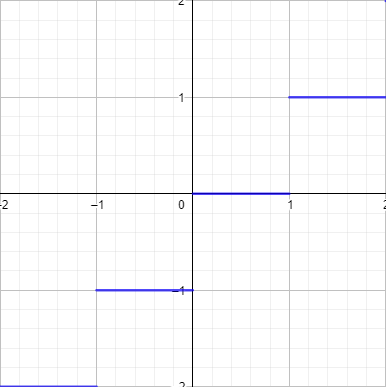
\includegraphics[scale=0.5]{images/partie_entiere.png}
	\caption{Partie entière}
\end{figure}

\begin{remarque}~
	\begin{itemize}
		\item E est croissante.
		\item E est non-continue en tout point de $\Z$.
		\item $x \mapsto x - E(x)$ est 1-périodique.
		\item $E^{-1}(\{0\}) = [0, 1[$.
	\end{itemize}
\end{remarque}


\section{Fonctions trigonométriques}
\begin{table}[h!]
	\centering
	\begin{tabular}{c c c c}
		\textbf{Fonction}
		& $f :\begin{cases}
			\R &\to \R \\    
			x &\mapsto \cos{x}
		\end{cases}$
		& $f :\begin{cases}
			\R &\to \R \\    
			x &\mapsto \sin{x}
		\end{cases}$
		& $f :\begin{cases}
			\R &\to \R \\    
			x &\mapsto \tan{x} = \frac{\sin{x}}{\cos{x}}
		\end{cases}$
		\\
		\hline
		\textbf{Parité} & Paire & Impaire & Impaire \\
		\textbf{Périodicité} & $2\pi\textnormal{-périodique}$ & $2\pi\textnormal{-périodique}$ & $\pi\textnormal{-périodique}$ \\
		\textbf{Dérivée} & $x \mapsto -\sin{x}$ & $x \mapsto \cos{x}$ & $x \mapsto \frac{1}{\cos^2{x}} = 1 + \tan^2{x}$ \\
		\textbf{Primitive} & $x \mapsto \sin{x}$ & $x\mapsto -\cos{x}$ & $x \mapsto - \ln{|\cos{x}|}$ \\
		\hline
	\end{tabular}
	\caption{Fonctions trigonométriques}
\end{table}


\begin{remarque}
	\par On peut éventuellement considérer l'ensemble d'arrivée de $\sin$ et $\cos$ comme étant $[-1,1]$
\end{remarque}


\begin{figure}[h!]
	\centering
	%\includegraphics{images/cos.png}
	\begin{subfigure}{0.3\textwidth}
\begin{tikzpicture}
            \begin{axis}[domain=-5:5, axis lines=middle, grid=both, xlabel=$x$, ylabel=$\cos(x)$, width=6cm]
                \addplot[color=green, samples=100] {cos(deg(x))};
            \end{axis}
    \end{tikzpicture}
		
		\caption{Fonction $\cos{x}$}
	\end{subfigure}
	\begin{subfigure}{0.3\textwidth}
\begin{tikzpicture}
            \begin{axis}[domain=-5:5, axis lines=middle, grid=both, xlabel=$x$, ylabel=$\sin(x)$, width=6cm]
                \addplot[color=green, samples=100] {sin(deg(x))};
            \end{axis}
    \end{tikzpicture}
		\caption{Fonction $\sin{x}$}
	\end{subfigure}
	\begin{subfigure}{0.3\textwidth}
\begin{tikzpicture}
            \begin{axis}[domain=-10:10, restrict y to domain=-10:10, axis lines=middle, grid=both, xlabel=$x$, ylabel=$\tan(x)$, width=6cm]
                \addplot[color=green, samples=100] {tan(deg(x))};
            \end{axis}
    \end{tikzpicture}
		\caption{Fonction $\tan{x}$}
	\end{subfigure}
\end{figure}

\begin{graybox}
	\begin{proposition}[Formules trigonométriques]
		$\forall x \in \R$ (il est possible de retrouver ces formules géométriquement)
		\begin{itemize}
			\item $\cos{x} = \cos{(-x)}$
			\item $\sin{(-x)} = -\sin{x}$
			\item $\cos{(\pi - x)} = -\cos{x}$
			\item $\sin{(\pi - x)} = \sin{x}$
			\item $\cos{(\pi + x)} = -\cos{x}$
			\item $\sin{(\pi + x)} = -\sin{x}$
			\item $\cos{(\frac{\pi}{2} - x)} = \sin{x}$
			\item $\sin{(\frac{\pi}{2} - x)} = \cos{x}$
			\item $\cos{(\frac{\pi}{2} + x)} = -\sin{x}$
			\item $\sin{(\frac{\pi}{2} + x)} = -\cos{x}$
		\end{itemize}
	\end{proposition}
\end{graybox}

% La base du code définissant le cercle trigonométrique provient de : https://texemple.net/tikz/exemples/unit-circle/
\begin{figure}[h!]
	\centering
	\begin{tikzpicture}[scale=3,cap=round,>=latex]
		% draw the coordinates
		\draw[->] (-1.5cm,0cm) -- (1.5cm,0cm) node[right,fill=white] {$x$};
		\draw[->] (0cm,-1.5cm) -- (0cm,1.5cm) node[above,fill=white] {$y$};
		
		% draw the unit circle
		\draw[thick] (0cm,0cm) circle(1cm);
		
		\foreach \x in {0,30,...,360} {
			% lines from center to point
			\draw[gray] (0cm,0cm) -- (\x:1cm);
			% dots at each point
			\filldraw[black] (\x:1cm) circle(0.4pt);
			% draw each angle in degrees
			\draw (\x:0.6cm) node[fill=white] {$\x^\circ$};
		}
		
		% draw each angle in radians
		\foreach \x/\xtext in {
			30/\frac{\pi}{6},
			45/\frac{\pi}{4},
			60/\frac{\pi}{3},
			90/\frac{\pi}{2},
			120/\frac{2\pi}{3},
			135/\frac{3\pi}{4},
			150/\frac{5\pi}{6},
			180/\pi,
			210/\frac{7\pi}{6},
			225/\frac{5\pi}{4},
			240/\frac{4\pi}{3},
			270/\frac{3\pi}{2},
			300/\frac{5\pi}{3},
			315/\frac{7\pi}{4},
			330/\frac{11\pi}{6},
			360/2\pi}
		\draw (\x:0.85cm) node[fill=white] {$\xtext$};
		
		\foreach \x/\xtext/\y in {
			% the coordinates for the first quadrant
			30/\frac{\sqrt{3}}{2}/\frac{1}{2},
			45/\frac{\sqrt{2}}{2}/\frac{\sqrt{2}}{2},
			60/\frac{1}{2}/\frac{\sqrt{3}}{2},
			% the coordinates for the second quadrant
			150/-\frac{\sqrt{3}}{2}/\frac{1}{2},
			135/-\frac{\sqrt{2}}{2}/\frac{\sqrt{2}}{2},
			120/-\frac{1}{2}/\frac{\sqrt{3}}{2},
			% the coordinates for the third quadrant
			210/-\frac{\sqrt{3}}{2}/-\frac{1}{2},
			225/-\frac{\sqrt{2}}{2}/-\frac{\sqrt{2}}{2},
			240/-\frac{1}{2}/-\frac{\sqrt{3}}{2},
			% the coordinates for the fourth quadrant
			330/\frac{\sqrt{3}}{2}/-\frac{1}{2},
			315/\frac{\sqrt{2}}{2}/-\frac{\sqrt{2}}{2},
			300/\frac{1}{2}/-\frac{\sqrt{3}}{2}}
		\draw (\x:1.25cm) node[fill=white] {$\left(\xtext,\y\right)$};
		
		% draw the horizontal and vertical coordinates
		% the placement is better this way
		\draw (-1.25cm,0cm) node[above=1pt] {$(-1,0)$}
		(1.25cm,0cm)  node[above=1pt] {$(1,0)$}
		(0cm,-1.25cm) node[fill=white] {$(0,-1)$}
		(0cm,1.25cm)  node[fill=white] {$(0,1)$};
	\end{tikzpicture}
	\caption{Cercle trigonométrique : \cite{cercle_trigo}}
\end{figure}
% Fin du code emprunté 



\begin{table}[h!]
	\centering
	\begin{tabular}{c c c c c c}
		$x$ & $0$ & $\frac{\pi}{6}$ & $\frac{\pi}{4}$ & $\frac{\pi}{3}$ & $\frac{\pi}{2}$ \\
		\hline
		$\cos{x}$ & 1 & $\frac{\sqrt{3}}{2}$ & $\frac{\sqrt{2}}{2}$ & $\frac{1}{2}$ & 0 \\
		$\sin{x}$ & 0 & $\frac{1}{2}$ & $\frac{\sqrt{2}}{2}$ & $\frac{\sqrt{3}}{2}$ & 1 \\
		$\sin^2{x}$ & 0 & $\frac{1}{4}$ & $\frac{2}{4}$ & $\frac{3}{4}$ & 1 \\ 
		\hline
	\end{tabular}
	\caption{Valeurs remarquables}
\end{table}

\begin{graybox}
	\begin{proposition}[Formules d'addition]
		$\forall (a, b) \in \R^2$
		\begin{align*}
			&\sin{(a+b)} = \sin{(a)}\cos{(b)} + \sin{(b)}\cos{(a)} \\
			&\cos{(a+b)} = \cos{(a)}\cos{(b)} - \sin{(a)}\sin{(b)}
		\end{align*}
	\end{proposition}
\end{graybox}

\begin{remarque}{En particulier pour $a=b$}~
	\begin{itemize}
		\item $\sin{(2a)} = 2 \sin{a}\cos{a}$
		\item $\cos{(2a)} = \cos^2{a}-\sin^2{a}$
		\item $\cos{(2a)} = 1 - 2\sin^2{a}$
		\item $\cos{(2a)} = 2\cos^2{a} - 1$
	\end{itemize}
	On en déduit :
	\begin{align*}
		\cos^2{a} &= \frac{1 + \cos{(2a)}}{2} & \sin^2{a} &= \frac{1 - \cos{(2a)}}{2}
	\end{align*}
\end{remarque}

\begin{remarque}[Mnémotechnique]~
	\\
	"cosinus est une fonction \textbf{raciste} et \textbf{menteuse}" 
	\begin{itemize}
		\item \textbf{Menteuse} : Elle change le signe
		\item \textbf{Raciste} : Elle ne mélange pas sinus et cosinus
	\end{itemize}
\end{remarque}

\section{Fonctions trigonométriques réciproques}
\begin{remarque}
	On cherche à changer l'ensemble de départ et d'arrivée pour rendre les fonctions trigonométriques bijectives.
\end{remarque}

\begin{graybox}
	\begin{proposition}[]
		Les fonctions :
		\begin{itemize}
			\item $\sin : [-\frac{\pi}{2}, \frac{\pi}{2}] \to [-1, 1]$
			\item $\cos : [0, \pi] \to [-1,1]$
			\item $\tan : ]-\frac{\pi}{2}, \frac{\pi}{2}[ \to \R$
		\end{itemize}
		sont bijectives.
	\end{proposition}
\end{graybox}

\begin{graybox}
	\begin{proposition}[]
		On peut définir leurs bijections réciproques :
		\begin{itemize}
			\item $\arcsin : [-1,1] \to [-\frac{\pi}{2},\frac{\pi}{2}]$
			\item $\arccos : [-1,1] \to [0, \pi]$
			\item $\arctan : \R \to ]-\frac{\pi}{2},\frac{\pi}{2}[$
		\end{itemize}
	\end{proposition}
\end{graybox}

\begin{graybox}
	\begin{proposition}[]
		On a alors : 
		\begin{itemize}
			\item $\forall x \in [-\frac{\pi}{2}, \frac{\pi}{2}], \arcsin{(\sin{x})} = x $
			\item $\forall x \in [0, \pi], \arccos{(\cos{x})} = x$
			\item $\forall x \in ]-\frac{\pi}{2}, \frac{\pi}{2}[, \arctan{(\tan{x})} = x$
		\end{itemize}
	\end{proposition}
\end{graybox}

\begin{graybox}
	\begin{proposition}[]
		\begin{align*}
			&\forall y \in [-1,1] 
			\begin{cases}
				\sin{(\arcsin{y})} = y \\
				\cos{(\arccos{y})} = y
			\end{cases}
			\\
			&\forall y \in \R \tan{(\arctan{y})} = y
		\end{align*}
	\end{proposition}
\end{graybox}

\begin{remarque}
	Les graphes des fonctions réciproques s'obtiennent par réflexion par rapport à la droite $y =x $
\end{remarque}

\begin{graybox}
	\begin{proposition}{Valeurs remarquables}
		\begin{itemize}
			\item $\arcsin{(1)} = \frac{\pi}{2}$
			\item $\arcsin{(0)} = 0$
			\item $\arcsin{(-1)} = -\frac{\pi}{2}$
			\item $\arccos{(1)} = 0$
			\item $\arccos{(0)} = \frac{\pi}{2}$
			\item $\arccos{(-1)} = \pi$
		\end{itemize}
	\end{proposition}
\end{graybox}

\begin{figure}[h!]
	\centering
	\begin{tikzpicture}
		\begin{axis}[domain=-1:1, axis lines=middle, grid=both, xlabel=$x$, ylabel=$y$, samples=100, legend pos=north west]
			\addplot[color=green]{x};
			\addlegendentry{$x$}
			\addplot[color=red]  {cos(deg(x))};
			\addlegendentry{$\cos(x)$}
			\addplot[color=blue]  {rad(acos(x))};
			\addlegendentry{$\arccos(x)$}
		\end{axis}
	\end{tikzpicture}
\end{figure}

\begin{figure}[h!]
	\centering
	\begin{tikzpicture}
		\begin{axis}[domain=-1:1, axis lines=middle, grid=both, xlabel=$x$, ylabel=$y$, samples=100, legend pos=north west]
			\addplot[color=green]{x};
			\addlegendentry{$x$};
			\addplot[color=red]  {sin(deg(x))};
			\addlegendentry{$\sin(x)$};
			\addplot[color=blue]  {deg(asin(x))};
			\addlegendentry{$\arcsin(x)$};
		\end{axis}
	\end{tikzpicture}
\end{figure}

\begin{figure}[h!]
	\centering
	\begin{tikzpicture}
		\begin{axis}[xmin=-5, xmax=5, ymin=-10, ymax=10, axis lines=middle, grid=both, xlabel=$x$, ylabel=$y$, samples=100, legend pos=north west]
			\addplot[color=green]{x};
			\addlegendentry{$x$};
			\addplot[color=red]  {tan(deg(x))};
			\addlegendentry{$\tan(x)$};
			\addplot[color=blue]  {rad(atan(x))};
			\addlegendentry{$\arctan(x)$};
		\end{axis}
	\end{tikzpicture}
\end{figure}


\begin{table}[h!]
	\centering
	\begin{tabular}{c c c c}
		\textbf{Fonction}& $\arcsin$ & $\arccos$ & $\arctan$ \\
		\hline
		\textbf{Monotonie} & Croissante & Décroissante & Croissante \\
		\textbf{Parité} & Impaire & $\emptyset$ & Impaire \\
		\hline
	\end{tabular}
	\caption{Monotonie et parité des fonctions trigonométriques réciproques}
\end{table}    

\begin{graybox}
	\begin{proposition}[Limite de $\arctan$]
		\begin{align*}
			\lim_{x \to +\infty}{\arctan{x}} &= \frac{\pi}{2} & \lim_{x \to -\infty}{\arctan{x}} &= -\frac{\pi}{2}
		\end{align*}
	\end{proposition}
\end{graybox}

\begin{graybox}
	\begin{proposition}[Dérivées]
		\begin{align*}
			1.\ \forall x \in ]-1, 1[ \ \arcsin'{x} = \frac{1}{\sqrt{1 - x^2}} 
		\end{align*}
		\begin{align*}
			2. \ \forall x \in [-1, 1] \ \arccos'{x} = - \frac{1}{\sqrt{1 - x^2}} 
		\end{align*}
		\begin{align*}
			3. \ \forall x \in \R \ \arctan'{x} = \frac{1}{1 + x^2}
		\end{align*}
	\end{proposition}
\end{graybox}

\begin{proof}
	1.
	\begin{align*}
		&\forall y \in [-1, 1] \textnormal{ on a : } \sin(\arcsin(y)) = y \\
		&\textnormal{Donc on a : } \cos^2(\arcsin(y)) + \underbrace{\sin^2(\arcsin(y))}_{=y^2} = 1 \\
		&\cos^2(\arcsin(y)) = 1 - y^2 \\
		&\arcsin(y) \in [-\frac{\pi}{2}, \frac{\pi}{2}] \textnormal{ donc } \cos(\arcsin(y)) > 0 \\
		&\textnormal{on en déduit } \cos(\arcsin(y)) = \sqrt{1 - y^2} \\
		&\textnormal{En dérivant on obtient : } \arcsin'(y) \times \underbrace{(-\sin(\arcsin(y)))}_{-y} = -\frac{2}{2\sqrt{1-y^2}} \\
		&\arcsin'(y)y = \frac{y}{\sqrt{1-y^2}} \\
		&y \neq 0,\ \arcsin'(y) = \frac{1}{\sqrt{1-y^2}}
	\end{align*}
\end{proof}

\begin{proof}
	2. Même principe que pour la 1.
\end{proof}

\begin{proof}
	3. $\forall x \in \R$
	\begin{align*}
		\tan\left(\arctan(x)\right) = x
	\end{align*}
	On a donc
	\begin{align*}
		&\arctan'(x) \tan'(\arctan(x)) = 1 \\
		\iff&\arctan'(x)(1 + \tan^2(\arctan(x))) = 1\\
		\iff&\arctan'(x) (1 + x^2) = 1 
	\end{align*}
	Comme $1 + x^2 > 0$ on en déduit :
	\begin{align*}
		\arctan'(x) = \frac{1}{1 + x^2}
	\end{align*}
\end{proof}

\section{Fonctions exponentielle et logarithme}

\begin{graybox}
	\begin{theoreme}[]
		Il existe une unique fonction dérivable $f:\R \to \R_+^*$ telle que :
		\begin{align*}
			\begin{cases}
				&\forall x \in \R, f'(x) = f(x) \\
				&f(0) = 1
			\end{cases}
		\end{align*}
		Cette fonction est la fonction exponentielle, notée :
		\begin{align*}
			\exp :
			\begin{cases}
				\R &\to \R^*_+ \\
				x &\mapsto \exp{(x)} \text{ ou } e^x     
			\end{cases}
		\end{align*}
	\end{theoreme}
\end{graybox}

\begin{graybox}
	\begin{proposition}[Monotonie de la fonction exponentielle]
		La fonction exponentielle est strictement croissante et $\exp{(0)} = 1$
	\end{proposition}
\end{graybox}

\begin{graybox}
	\begin{proposition}[Limites de la fonction exponentielle]
		\begin{align*}
			\lim_{x \to -\infty} \exp{(x)} &= 0 & \lim_{x \to +\infty} \exp{(x)} &= +\infty
		\end{align*}
	\end{proposition}
\end{graybox}

\begin{graybox}
	\begin{proposition}[Propriétés de la fonction exponentielle]
		$\forall x \in \R, \forall y \in \R$
		\begin{itemize}
			\item $\exp{(x+y)} = \exp{(x)} \times \exp{(y)}$
			\item $\exp{(x - y)} = \frac{\exp{(x)}}{\exp{(y)}}$
			\item $\exp{(-x)} = \frac{1}{\exp{(x)}}$
		\end{itemize}    
	\end{proposition}
\end{graybox}

\begin{graybox}
	\begin{definition}[Logarithme néperien]
		La fonction exponentielle est bijective, on définit sa bijection réciproque :
		\begin{align*}
			\ln : 
			\begin{cases}
				\R^*_+ &\to \R \\
				x &\mapsto \ln{(x)}        
			\end{cases}
		\end{align*}
		$\forall x \in \R^*_+, \ln{(x)}$ est l'unique réel tel que $\exp{\left(\ln{\left(x \right)}\right)} = x$ \\
		On a aussi $\forall y \in \R, \ln{(\exp{(y)})} = y$.
	\end{definition}
\end{graybox}


\begin{graybox}
	\begin{proposition}[Monotonie du logarithme néperien]
		La fonction logarithme néperien est croissante et $\ln{(1)} = 0$.    
	\end{proposition}
\end{graybox}

\begin{graybox}
	\begin{proposition}[Limites du logarithme néperien]
		\begin{align*}
			\lim_{x \to 0} \ln{(x)} &= -\infty & \lim_{x \to +\infty} \ln{(x)} &= +\infty
		\end{align*}
	\end{proposition}
\end{graybox}

\begin{graybox}
	\begin{proposition}[Propriétés fondamentales]
		$\forall (x,y) \in (\R^*_+)^2$
		\begin{itemize}
			\item $\ln(xy) = \ln(x) + \ln(y)$
			\item $\ln(\frac{1}{x}) = -\ln(x)$
			\item $\ln(\frac{x}{y}) = \ln(x) - \ln(y)$
			\item $\ln(x^n) = n \ln(x)$
		\end{itemize}
	\end{proposition}
\end{graybox}

\begin{graybox}
	\begin{proposition}[Dérivée de la fonction $\ln$]
		La fonction $\ln$ est dérivable sur $\R^*_+$ et $\forall x \in \R^*_+, \ln'(x) = \frac{1}{x}$
	\end{proposition}
\end{graybox}

\begin{proof}
	On dérive la relation $\exp(\ln(x)) = x$
	\begin{align*}
		&\ln'(x) \exp'(\ln(x)) = 1 \\
		&\ln'(x) \exp(\ln(x)) = 1 \\
		&\ln'(x) x = 1 \\
		&\ln'(x) = \frac{1}{x}
	\end{align*}
\end{proof}

\begin{figure}[!h]
	\centering
	\begin{subfigure}{0.45\textwidth}
		\begin{tikzpicture}
			\begin{axis}[domain=0:5, axis lines=middle, grid=both, xlabel=$x$, ylabel=$e^x$, width=7cm]
				\addplot[color=red, samples=50]{e^x};
			\end{axis}
		\end{tikzpicture}  
		\caption{Fonction exponentielle}
	\end{subfigure}
	\begin{subfigure}{0.45\textwidth}
		\begin{tikzpicture}
			\begin{axis}[domain=0:10, axis lines=middle, grid=both, xlabel=$x$, ylabel=$\ln(x)$, width=7.5cm]
				\addplot[color=red, samples=100]{ln(x)};
			\end{axis}
		\end{tikzpicture}
		\caption{Fonction logarithme népérien}
	\end{subfigure}
\end{figure}

\section{Fonctions hyperboliques}
\begin{graybox}
	\begin{definition}[Fonctions hyperboliques]
		On définit $\forall x \in \R$ 
		\begin{align*}
			\cosh(x) &= \frac{e^x + e^{-x}}{2} & \sinh(x) &= \frac{e^x - e^{-x}}{2} & \tanh(x) &= \frac{\sinh(x)}{\cosh(x)} = \frac{e^x - e^{-x}}{e^x + e^{-x}}
		\end{align*}
	\end{definition}
\end{graybox}

\begin{remarque}
	$\cosh = \mathrm{ch},\ \sinh = \mathrm{sh},\ \tanh = \mathrm{th}$
\end{remarque}

\begin{figure}[htbp]
	\centering
	\begin{subfigure}{0.3\textwidth}
		%\includegraphics[width=\textwidth, height=3.5cm]{images/ch.png}
		
		\begin{tikzpicture}
			\begin{axis}[domain=-5:5, axis lines=middle, grid=both, xlabel=$x$, ylabel=$\cosh(x)$, width=5cm]
				\addplot[color=red, samples=100]  {cosh(x)};
			\end{axis}
		\end{tikzpicture}
		\caption{Fonction cosh \cite{graphes}}
	\end{subfigure}
	\begin{subfigure}{0.3\textwidth}
		%\includegraphics[width=\textwidth, height=3.5cm]{images/sh.png}
		\begin{tikzpicture}
			\begin{axis}[domain=-5:5, axis lines=middle, grid=both, xlabel=$x$, ylabel=$\sinh(x)$, width=5cm]
				\addplot[color=red, samples=100]  {sinh(x)};
			\end{axis}
		\end{tikzpicture}
		\caption{Fonction sinh \cite{graphes}}
	\end{subfigure}
	\begin{subfigure}{0.3\textwidth}
		%\includegraphics[width=\textwidth, height=3.5cm]{images/tanh.png}
		\begin{tikzpicture}
			\begin{axis}[domain=-5:5, axis lines=middle, grid=both, xlabel=$x$, ylabel=$\tanh(x)$, width=5cm]
				\addplot[color=red, samples=100]  {tanh(x)};
			\end{axis}
		\end{tikzpicture}
		\caption{Fonction tanh \cite{graphes}}
	\end{subfigure}
\end{figure}

\begin{table}[h!]
	\centering
	\begin{tabular}{c c c c}
		Fonction & ch & sh & th \\
		\hline
		Domaine de définition & $\R$ & $\R$ & $\R$ \\
		Parité & paire & impaire & impaire \\
		Dérivée & sh & ch & $1 - \mathrm{th}^2$ \\
		$\lim_{+\infty}$ & $+\infty$ & $+\infty$ & 1 \\
		$\lim_{-\infty}$ & $+\infty$ & $-\infty$ & -1 \\
		\hline
	\end{tabular}
\end{table}

\begin{graybox}
	\begin{proposition}[]
		$\forall x \in \R$
		\begin{align*}
			\cosh^2(x) - \sinh^2(x) = 1
		\end{align*}
	\end{proposition}
\end{graybox}

\begin{proof}
	\begin{align*}
		\cosh^2(x) - \sinh^2(x) &= \left( \frac{e^x + e^{-x}}{2} \right)^2 - \left( \frac{ e^x - e^{-x} }{ 2 } \right)^2 \\
		&= \frac{e^{2x} + 2 + e^{-2x} - (e^{2x} - 2 + e^{-2x})}{4} \\
		&= \frac{4}{4} \\
		&= 1
	\end{align*}
\end{proof}

\begin{graybox}
	\begin{proposition}[]
		$\forall x \in \R$
		\begin{align*}
			\tanh'(x) = 1 - \tanh^2(x)
		\end{align*}
	\end{proposition}
\end{graybox}

\begin{proof}
	$\tanh = \frac{\sinh}{\cosh}$
	\begin{align*}
		\tanh'(x) &= \frac{\sinh'(x)\cosh(x) - \sinh(x)\cosh'(x)}{\cosh^2(x)} \\
		&= \frac{\cosh^2(x) - \sinh^2(x)}{\cosh^2(x)} \\
		&= \frac{1}{\cosh^2(x)} = 1 - \tanh^2(x)
	\end{align*}
\end{proof}

\begin{graybox}
	\begin{proposition}[]
		$\forall x \in \R$ 
		\begin{align*}
			&\cosh{(x)} + \sinh{(x)} = \exp{(x)} \\
			&\cosh{(x)} - \sinh{(x)} = \exp{(-x)}
		\end{align*}
		On dit que $\cosh$ est la partie paire et $\sinh$ la partie impaire de l'exponentielle.
	\end{proposition}
\end{graybox}

\begin{graybox}
	\begin{proposition}[]
		$\forall (x, y) \in \R^2$
		\begin{align*}
			&1.\cosh{(x + y)} = \cosh{(x)}\cosh{(y)} + \sinh{(x)}\sinh{(y)} \\
			&2.\sinh{(x + y)} = \cosh{(x)}\sinh{(y)} + \sinh{(x)}\cosh{(y)}
		\end{align*}
	\end{proposition}
\end{graybox}

\begin{proof}
	1. 
	\begin{align*}
		\cosh{(x)}\cosh{(y)} + \sinh{(x)}\sinh{(y)} &= \left( \frac{e^x + e^{-x}}{2} \right) \left( \frac{e^y + e^{-y}}{2} \right) + \left( \frac{e^x - e^{-x}}{2} \right) \left( \frac{e^y - e^{-y}}{2} \right)\\
		&= \frac{e^x e^y + e^x e^{-y} + e^{-x}e^y + e^{-x} e^{-y}}{4} + \\ &\quad \frac{e^x e^y - e^x e^{-y} - e^{-x}e^y + e^{-x}e^{-y}}{4} \\
		&= \frac{2e^{x+y} + 2e^{-x-y}}{4} \\
		&= \frac{e^{x+y} + e^{-x-y}}{2} \\
		&= \cosh{(x + y)}
	\end{align*}
\end{proof}

\begin{remarque}
	En prenant $y = x$ on obtient :
	\begin{align*}
		\cosh{(2x)} &= \cosh^2{(x)} + \sinh^2{(x)} \\
		&= 1 + 2 \sinh^2{(x)} \\
		&= 2\cosh^2{(x)} - 1 \\
		\sinh{(2x)} &= 2\cosh{(x)} \sinh{(x)}
	\end{align*}
\end{remarque}


\begin{remarque}
	On verra avec les complexes :
	\begin{align*}
		\cos{x} &= \frac{e^{ix} + e^{-ix}}{2} & \sin{x} &= \frac{e^{ix} - e^{-ix}}{2}
	\end{align*}
	qui expliquent la parenté entre $\cos / \cosh$ et $\sin / \sinh$
\end{remarque}

\section{Fonctions puissance}
\par Dans quel cas peut-on définir $x^a$ ?

\begin{enumerate}
	\item Si $a \in \N, \forall x \in \R$
	\begin{align*}
		x^a = \underbrace{x \times x \times \cdots x}_{a \ fois}
	\end{align*}
	Par convention $x^0 = 1$
	\begin{align*}
		\begin{cases}
			\mathbb{R} &\to \mathbb{R} \\
			x &\mapsto x^a 
		\end{cases}
	\end{align*}
	est la fonction polynomiale de même parité que $a$.
	\item Si $a \in \mathbb{Z} \backslash \mathbb{N}$ et $x \neq 0$
	On pose 
	\begin{align*}
		x^a = \frac{1}{x^{-a}}
	\end{align*}
	\item Si $a = \frac{1}{n}$ pour $n \in \mathbb{N}^*$
	\begin{itemize}
		\item est la racine n-ième de $x$
		\item  $x^a$ est toujours défini quand $x \geqslant 0$, comme l'unique $y \in \mathbb{R}^+$ tel que $y^n = x$
		\item Si $n$ est impair : $x^a$ est défini pareillement pour tout $x \in \mathbb{R}$
	\end{itemize}
	\item Si $a \in \mathbb{R}$ et $x \in ]0, +\infty[$
	On pose : $x^a = \exp{(a \ln{x})}$ \\
	Les propriétés suivantes sont vraies dans tous les cas : 
	\begin{itemize}
		\item $1^a = 1$
		\item $x^a \cdot x^b = x^{a+b}$
		\item $(xy)^a = x^a y^a$
		\item $(x^a)^b = x^{ab}$
	\end{itemize}
	Si $x = e$, on retrouve la formule : $\exp{(a)}^b = \exp{(ab)}$
\end{enumerate}

\begin{graybox}
	\begin{proposition}[Dérivée de la fonction puissance]
		Soit la fonction :
		\begin{align*}
			f :
			\begin{cases}
				\mathbb{R}^*_+ &\to \mathbb{R} \\
				x &\mapsto x^a
			\end{cases}
		\end{align*}
		$f$ est dérivable et :
		\begin{align*}
			f'(x) &= \frac{a}{x} \exp{(a\ln{a})}  \\
			&= a x^{-1}x^a  \\
			&= a x^{a - 1}
		\end{align*}    
	\end{proposition}
\end{graybox}

\begin{exemple}
	Quelle est la dérivée de $g : x \mapsto 2^x$ ? \\
	On a : $g(x) = \exp{(x \ln{(2)})}$
	\begin{align*}
		g'(x) &= \ln{(2)} \exp{(x\ln{(2)})} \\
		g'(x) &= \ln{2} \cdot 2^x
	\end{align*}
\end{exemple}

\begin{graybox}
	\begin{theoreme}[Croissances comparées]
		$\forall (a, b) \in (\R^*_+)^2$
		\[\lim_{x \to +\infty} \frac{\exp{(ax)}}{x^b} = + \infty \]
		\[\lim_{x \to +\infty} \frac{x^a}{(\ln{x})^b} = +\infty\] 
		\[\lim_{x \to +\infty} \frac{\exp{(ax)}}{(\ln{x})^b} = +\infty\]
		\[ \lim_{x \to -\infty} |x|^b \exp{(ax)} = 0 \]
		\[ \lim_{x \to +\infty} \frac{(\ln{(x)})^b}{x^a} = 0 \]
		\[ \lim_{x \to 0^{+}} x^a |\ln{(x)}|^b = 0 \]
	\end{theoreme}
\end{graybox}
cd 
\chapter{Suites réelles}
\section{Définitions}

\begin{graybox}
    \begin{definition}[Suite réelle]
\par On appelle \textbf{suite réelle} une fonction de $\N \to \R$. On note $(u_n)_{n \in \N}$ la fonction $x \mapsto u_n$
\end{definition}
\end{graybox}

\begin{exemple}
\par On définit la suite $(u_n)_{n \in \N}$ par la formule 
\begin{align*}
    \forall n \in \N, u_n = 3n + 7
\end{align*}

\begin{itemize}
    \item $u_0 = 7$
    \item $u_1 = 10$
    \item $u_2 = 13$
\end{itemize}
\end{exemple}

\begin{remarque}
\par On met des parenthèses pour parler de la suite dans son intégralité. On ne met pas de parenthèses pour parler d'un seul terme de la suite.
\end{remarque}

\begin{remarque}
    \par On peut définir une suite par récurrence.
\end{remarque}

\begin{exemple}
    \begin{align*}
        \forall n \geqslant 1 :
        \begin{cases}
        u_0 = 2 \\
        u_n = \frac{1}{n} + \frac{u_{n - 1}}{3}
        \end{cases}
    \end{align*}
\end{exemple}

\begin{remarque}
    Le vocabulaire des fonctions s'applique aussi aux suites.
\end{remarque}

\begin{graybox}
    \begin{definition}[Monotonie d'une suite]
    \par Soit $(u_n)_{n \geqslant 0}$ une suite. 
    \begin{itemize}
        \item On dit que $(u_n)_{n  \geqslant 0}$ est \textbf{croissante} si $\forall n \in \mathbb{N}, u_n \leqslant u_{n + 1}$
        \item On dit que $(u_n)_{n \geqslant 0}$ est \textbf{décroissante} si $\forall n \in \mathbb{N}, u_n \geqslant u_{n+1}$
        \item $(u_n)_{n \geqslant 0}$ est \textbf{majorée} si $\exists M \in \mathbb{R}, \forall n \in \mathbb{N}, u_n \leqslant M$
        \item $(u_n)_{n \geqslant 0}$ est \textbf{minorée} si $\exists m \in \mathbb{R}, \forall n \in \mathbb{N}, u_n \geqslant m$
        \item $(u_n)_{n \geqslant 0}$ est \textbf{bornée} si elle est majorée et minorée $\iff \exists M \in \mathbb{R}, \forall n \in \mathbb{N}, |u_n| \leqslant M$
    \end{itemize}
\end{definition}
\end{graybox}

\begin{remarque}
    \par Une suite $(u_n)_{n \geqslant 0}$ est croissante $\iff$ $\forall (m,n) \in \mathbb{N}^2, m \leqslant n \implies u_m \leqslant u_n$
    On dit aussi que $(u_n)_{n \geqslant 0}$ est monotone si elle est croissante ou décroissante.
\end{remarque}

\begin{remarque}
    \par L'ensemble d'indices est parfois $\mathbb{N}^*$ plutôt que $\mathbb{N}$, d'où la suite $(u_n)_{n \geqslant 1}$.
    On peut aussi avoir $(u_n)_{n \geqslant 2}$. Les résultats du cours seront énoncés par des suites $(u_n)_{n \geqslant 0}$ mais aussi valables pour des suites $(u_n)_{n \geqslant 1}$
\end{remarque}

\begin{remarque}
    \par Soit $P(x)$ une propriété qui dépend de $n \in \mathbb{N}$. On dit que $P(n)$ est vraie \textbf{à partir d'un certain rang}, si $\exists n_0 \in \mathbb{N}, \forall n \geqslant n_0$, $P(n)$ est vraie.
\end{remarque}

\begin{exemple}
    \par Soit $(u_n)_{n \geqslant 0}$ définie par $\forall n \in \mathbb{N}, u_n = 2^n - 10n$
    \begin{itemize}
        \item $u_0 = 1$
        \item $u_1 = -8$
        \item $u_2 = -16$
        \item $u_3 = -22$
    \end{itemize}
    \par La suite $(u_n)_{n \geqslant 0}$ n'est pas croissante. Mais elle est croissante à partir d'un certain rang.
    \begin{align*}
        \forall n \in \mathbb{N}, u_{n+1} - u_n &= 2^{n+1} - 10(n+1) - 2^n + 10n \\
        &= u_{n+1} - u_n = 2 \cdot 2^n - 2^n - 10 \\
        &= u_{n + 1} - u_n = 2^n - 10 \text{ qui est } \geqslant 0 \text{ pour } n \geqslant 4
    \end{align*}
\end{exemple}

\begin{graybox}
    \begin{proposition}[Propriétés des suites]
    \par Soient $(u_n)_{n \geqslant 0} \text{ et } (v_n)_{n \geqslant 0}$ deux suites. On peut former :
    \begin{itemize}
        \item La somme : $(u_n + v_n)_{n \geqslant 0}$
        \item Le produit : $(u_n v_n)_{n \geqslant 0}$
        \item Pour $\lambda \in \mathbb{R}, (\lambda u_n)_{n \geqslant 0}$
    \end{itemize}
\end{proposition}
\end{graybox}

\subsection{Suites classiques}

\begin{graybox}
    \begin{proposition}[Suite arithmétique]
    Suite arithmétique de progression $r \in \R$ donnée par $u_0 \in \mathbb{R}$ est la relation de récurrence $u_{n+1} = u_n + r, \forall n \in \mathbb{N}$. On a alors pour tout $n \in \mathbb{N}$
    \begin{align*}
        u_n = u_0 + nr
    \end{align*}
    On peut aussi calculer :
    \begin{align*}
        \sum_{k = 0}^{n} u_k &= \sum_{k=0}^{n} (u_0 + kr) \\
        &= (n+1) u_0 + r\sum_{k=0}^{n}k \\
        &= (n+1)u_0 + r \frac{n(n+1)}{2}
    \end{align*}
\end{proposition}
\end{graybox}

\begin{graybox}
    \begin{proposition}[Suite géométrique]
    Suite géométrique de raison $q \in \R^*$ donnée par $u_0 \in \mathbb{R}$ et la relation de récurrence $u_{n+1} = q u_n, \forall n \in \mathbb{N}$
	       On a alors $\forall n \in \mathbb{N}, u_n = u_0 q^n$
	       On peut aussi calculer :
        	\begin{align*}
        	\sum_{k=0}^{n}u_k &= \sum_{k=0}^{n} u_0 q^k \\
        					  &= u_0 \sum_{k=0}^{n}q^k	
        	\end{align*}        
            Sachant que : 
            \begin{align*}
                	\sum_{k=0}^{n} q^k = \frac{1 - q^{n+1}}{1 - q}, \ q\neq 1
            \end{align*}
            On a :
            	\begin{align*}
            	&\text{Si }q\neq 1 :  \sum_{k=0}^{n}u_k = u_0 \frac{1 - q^{n+1}}{1 - q} \\
            	&\text{Si } q = 1 : \sum_{k=0}^{n}u_k = (n+1)u_0
            	\end{align*}
\end{proposition}
\end{graybox}

\begin{graybox}
    \begin{proposition}[Suite arithmético-géométrique]
    Suites arithmético-géométrique de progression $r \in \mathbb{R}$ et de raison $q \in \mathbb{R^*}$ donnée par $u_0 \in \mathbb{R}$ et $\forall n \in \mathbb{N}, u_{n+1} = qu_n + r$ Comment calculer $u_n$ ?
        \begin{itemize}
            \item Si $q = 1$ c'est une suite arithmétique
            \item Si $q \neq 1$, on cherche le réel $a$ tel que $a = q a + r$ et on regarde la suite $(u_n - a)_{n \geqslant 0}$
            	 \begin{align*}
                	 a = qa + r &\iff a - qa = r \\
                	            &\iff a = \frac{r}{1 - q} \text{ (Possible 
                 car } q\neq 1)
              \end{align*} 
              
              $\forall n \in \N$ :
              	\begin{align*}
            	u_{n+1} &= qu_n + r \\
            	u_{n+1} - a &= qu_n + r - a \\
            	v_{n+1} &= q(v_n + a) + r - a \\
            	        &= qv_n + \underbrace{qa + r - a}_{=0}
            	\end{align*}
             Ainsi $(v_n)_{n \geq 0}$ est une suite géométrique de raison $q$, donc $\forall n \in \N$
             	\begin{align*}
            	v_n &= v_0 q^n \\
            	    &= (u_0 - a) q^n
            	\end{align*}
              et 
                  \begin{align*}
                    u_n &= v_n + a \\
                    u_n &= a + (u_0 - a)q^n
                    \end{align*}
        \end{itemize}   
\end{proposition}
\end{graybox}

\section{Convergence d'une suite}

\begin{graybox}
    \begin{definition}[]
    \par Soit $(u_n)_{n \geqslant 0}$ une suite et $l \in \mathbb{R}$. On dit que la suite $(u_n)_{n \geqslant 0}$ tend vers $l$ si :
    \begin{align*}
    \forall \varepsilon > 0,\ \exists N \in \mathbb{N},\ \forall n \in \mathbb{N},\ |u_n - l| \leqslant \varepsilon
    \end{align*}
    \par On note alors :
    \begin{align*}
    u_n \xrightarrow[n \to +\infty]{}l \ \text{ ou }\lim_{n \to +\infty} u_n = l
    \end{align*}
\end{definition}
\end{graybox}



    \begin{remarque}
    $\varepsilon$ : epsilon s'utilise pour un réel > 0 petit
\end{remarque}



    \begin{remarque}
    La valeur de N dépend de $\varepsilon$ car le $\exists$ vient après le $\forall$
\end{remarque}



    \begin{remarque}
    $|u_n - l| \leqslant \varepsilon$ revient à dire que $-\varepsilon \leqslant u_n - l \leqslant \varepsilon$
    ou encore $l - \varepsilon \leqslant u_n \leqslant l + \varepsilon$
    ou bien $u_n \in [l - \varepsilon, l + \varepsilon]$
    Ainsi, dire que  $\displaystyle{\lim_{n \to +\infty} u_n = l}$ revient à dire que tout intervalle $[l-\varepsilon, l + \varepsilon]$ contient les termes de $(u_n)_{n \geqslant 0}$ à partir d'un certain rang.
\end{remarque}



    \begin{exemple}
    La suite $(u_n)_{n \geqslant 0}$ définie par $u_n = \frac{1}{n+1}, \forall n \in \mathbb{N}$ tend vers 0.
\end{exemple}



    \begin{proof}
    Soit $\varepsilon > 0$ 
	Si $l = 0$
	\begin{align*}
	|u_n - l| \leqslant \varepsilon &\iff \left| \frac{1}{n+1} \right| \leqslant \varepsilon \\
	&\iff \frac{1}{n+1} \leqslant \varepsilon \\
	&\iff \frac{1}{\varepsilon} \leqslant n + 1
	\end{align*}
    Posons $N = E(\frac{1}{\varepsilon})$ alors $N \leqslant \frac{1}{\varepsilon} < N + 1$
    et alors : 
    \begin{align*}
        \forall n \geqslant N, n + 1 \geqslant N + 1 > \frac{1}{\varepsilon}
    \end{align*}
    donc $n + 1 \geqslant \frac{1}{\varepsilon}$ et $|u_n - l| < \varepsilon$
    On a bien vérifié que $\displaystyle{\lim_{n \to +\infty} u_n = 0}$
    \end{proof}


    \begin{remarque}
    Pour démontrer une assertion de type $\forall \varepsilon > 0 \ldots$ on commence par "Soit $\varepsilon > 0$" 
\end{remarque}



    \begin{exemple}
    Soit $(u_n)_{n \geqslant 0}$ définie par :
    \begin{align*}
        u_n =
        \begin{cases}
            0 \ &\text{ si n pair } \\
            \frac{1}{n} \ &\text{ si n impair}
        \end{cases}
    \end{align*}
    La suite tend vers 0
    \begin{proof}
        Soit $\varepsilon > 0$
        Posons : $N = E \left(\frac{1}{\varepsilon} \right) + 1$, alors $\frac{1}{\varepsilon} \leqslant N$
        \\
        Soit $n \geqslant N$
        \begin{itemize}
            \item Si n est pair : $\left| u_n - 0 \right| = 0 < \varepsilon$
            \item Si n est impair : $\left|u_n - 0 \right| = \frac{1}{n} < \frac{1}{N} \leqslant \varepsilon$
        \end{itemize}
        Et donc $\displaystyle{\lim_{n \to +\infty} u_n = 0}$
    \end{proof}
\end{exemple}

\begin{graybox}
    \begin{definition}[]
    On dit que $(u_n)_{n \geqslant 0}$ converge si $\exists l \in \mathbb{R} \backslash \{\pm\infty\}$ tel que $\displaystyle{\lim_{n \to +\infty} u_n = l}$
    \begin{align*}
        (u_n)_{n \geqslant 0} \text{ converge} \iff \exists l \in \mathbb{R}, \forall \varepsilon > 0, \exists N \in \mathbb{N}, \forall n \geqslant, \left|u_n - l\right| \leqslant \varepsilon
    \end{align*}
    Sinon on dit que $(u_n)_{n \geqslant 0}$ diverge
    \begin{align*}
        (u_n)_{n \geqslant 0} \text{ diverge } \iff \forall l \in \mathbb{R}, \exists \varepsilon > 0, \forall N \in \mathbb{N}, \exists n \geqslant N, \left|u_n - l\right| > \varepsilon
    \end{align*}
    \begin{align*}
        (u_n)_{n \geqslant 0} \text{ ne converge pas vers l } &\iff \exists \varepsilon > 0, \forall N \in \mathbb{N}, \exists n \geqslant N, |u_n - l| > \varepsilon \\
        &\iff \exists \varepsilon > 0, \{n \in \mathbb{N} \text{ tq } |u_n - l| > \varepsilon\} \\ &\text{ est un ensemble infini}
    \end{align*}
    \begin{align*}
        \lim_{n \to +\infty} = l \iff \forall \varepsilon > 0 \{n \in \mathbb{N}, |u_n - l| > \varepsilon\} \text{ est fini }
    \end{align*}
\end{definition}
\end{graybox}

\begin{exemple}
    Soit $(u_n)_{n \geqslant 0}$ définie par 
    \begin{align*}
        u_n = (-1)^n =
        \begin{cases}
        1 &\text{ si n pair} \\
        -1 &\text{ si n impair}
        \end{cases}
    \end{align*}
    Cette suite diverge. \\
    En effet, soit $l \in \mathbb{R}$
    \begin{itemize}
        \item Si $l < 0$
        \begin{align*}
            |u_n - l| = |1 - l| \geqslant 1
        \end{align*}
        quand n est pair et donc aucun nombre pair n vérifie
        \begin{align*}
            |u_n - l| \leqslant \frac{1}{2}
        \end{align*}
        et donc $(u_n)_{n \geqslant 0}$ ne converge pas vers $l$
        puisque l'ensemble  
        \begin{align*}
            \left\{n \in \mathbb{N}, |u_n - l| > \frac{1}{2}\right\}
        \end{align*}
        est infini.
        
        \item Si $l > 0$, de même $|u_n - l| \geqslant 1$ pour n impair et donc $(u_n)_{n \geqslant 0}$ ne converge pas vers $l$
    \end{itemize}
\end{exemple}

\begin{graybox}
    \begin{theoreme}[Unicité de la limite]
    La limite d'une suite convergente $(u_n)_{n \in \N}$ est unique. Pour $\forall (l_1, l_2) \in \R^2$
    \begin{align*}
        \text{Si } \lim_{n \to +\infty} u_n = l_1 \text{ et }\lim_{n \to +\infty} u_n = l_2 \text{ alors } l_1 = l_2
    \end{align*}
\end{theoreme}
\end{graybox}


\begin{proof}
         \par Procédons à un raisonnement par l'absurde. \\
         \par \noindent On suppose que $l_1 \neq l_2$. Posons $\varepsilon = \frac{1}{3} |l_1 - l_2| > 0$. \\
         D'après la définition de limite :
         \begin{align*}
             &\exists N_1 \in \N, \forall n \geq N_1, |u_n - l_1| \leq \varepsilon \\
             &\exists N_2 \in \N, \forall n \geq N_2, |u_n - l_2| \leq \varepsilon
         \end{align*}
         \par \noindent Posons $N = \max(N_1, N_2)$ Si $n \geq N$ alors :
         \begin{align*}
             &|u_n - l_1| \leq \varepsilon \\
             &|u_n - l_2| \leq \varepsilon
         \end{align*}
         \par \noindent Alors $|l_1 - l_2| \leq |u_n - l_1| + |u_n + l_2| \leq \varepsilon + \varepsilon = 2\varepsilon = \frac{2}{3}|l_1 - l_2|$.
    On en déduit $\frac{1}{3}|l_1 - l_2| \leq 0$, ce qui est absurde. Ainsi, on a montré que $l_1 = l_2$
\end{proof}

\begin{graybox}
    \begin{theoreme}[]
    Toute suite convergente est bornée.
\end{theoreme}
\end{graybox}

\begin{proof}
        \par \noindent Supposons qu'une suite $(u_n)_{n \geq 0}$ converge vers $\ell \in \R$. 
        \par \noindent On applique la définition de convergence avec $\varepsilon = 1$
        \begin{align*}
            \exists N \in \N, \forall n \geq N, |u_n - \ell| \leq 1 \vee \ell - 1 \leq u_n \leq \ell + 1
        \end{align*}
        \par \noindent Posons $M = \max(u_0, u_1, \ldots, u_{N - 1}, \ell + 1)$ et $m = \min(u_0, u_1, \ldots, u_{N -1}, \ell - 1)$.
        \begin{align*}
            &\forall n \in \N \\
            &\textnormal{Si } n < N, m \leq u_n \leq M \\
            &\textnormal{Si } n > N, m \leq \ell - 1 \leq u_n \leq \ell + 1 \leq M
        \end{align*}
        $(u_n)_{n \geq 0}$ est majorée par $M$ et minorée par $m$, elle est donc bornée.
    \end{proof}

\begin{remarque}
    La réciproque n'est pas vraie, il existe des suites bornées non convergentes comme par exemple : $u_n = (-1)^{n}$
\end{remarque}

\subsection{Opérations sur les suites convergentes}

\begin{graybox}
    \begin{theoreme}[]
    \par \noindent Soient $(u_n)_{n \geq 0}$ et $(v_n)_{n \geq 0}$ deux suites convergentes. \\
    On suppose que
    \begin{align*}
        \lim_{n \to +\infty} u_n = \ell_1, \lim_{n \to +\infty} v_n = \ell_2, (\ell_1, \ell_2) \in \R^2
    \end{align*}
    Pour $(\alpha, \beta) \in \R^2$, $(\alpha u_n + \beta v_n)_{n \geq 0}$ converge vers $\alpha \ell_1 + \beta \ell_2$.
\end{theoreme}
\end{graybox}

\begin{proof}
        Soit $\varepsilon > 0$ \\
        Posons : 
        \begin{align*}
            \varepsilon ' = \frac{\varepsilon}{|\alpha| + |\beta|} > 0, \textnormal{ avec } |\alpha| + |\beta| > 0
        \end{align*}
        \par \noindent Par définition de la limite :
        \begin{align*}
            &\exists N_1 \in \N, \forall n \geq N_1, |u_n - \ell_1| \leq \varepsilon' \\
            &\exists N_2 \in \N, \forall n \geq N_2, |v_n - \ell_2| \leq \varepsilon'
        \end{align*}
        Posons $N = \max(N_1, N_2)$. Si $n \geq N$, alors :
        \begin{align*}
            |u_n - \ell_1| \leq \varepsilon' \textnormal{ et } |v_n - \ell_2| \leq \varepsilon'
        \end{align*}
        Alors
        \begin{align*}
        |\alpha u_n + \beta v_n - (\alpha \ell_1 + \beta \ell_2)| &= |\alpha(u_n - \ell_1) + \beta(v_n - \ell_2)| \\
        & \leq |\alpha| |u_n - \ell_1| + |\beta| |v_n - \ell_2| \\
        &\leq (|\alpha| + |\beta|)\varepsilon' = \varepsilon 
        \end{align*}
        On a montré que $\alpha u_n + \beta v_n$ converge vers $\alpha \ell_1 + \beta \ell_2$.
    \end{proof}

\begin{remarque}
    En particulier : 
    \begin{align*}
        (u_n)_{n \geq 0} \textnormal{ convergente et } (v_n)_{n \geq 0} \textnormal{ convergente } \implies (u_n + v_n)_{n \geq 0} \textnormal{ convergente} 
    \end{align*}
    La réciproque est fausse : \\
    $u_n = n \textnormal{ divergente}$ et $v_n = -n \textnormal{ divergente}$ mais $u_n + v_n = 0$ convergente.
\end{remarque}

\begin{graybox}
    \begin{theoreme}[]
    Soient $(u_n)_{n \geq 0}$ et $(v_n)_{n \geq 0}$ deux suites convergentes. On suppose que :
    \begin{align*}
        \lim_{n \to +\infty} u_n = \ell_1, \lim_{n \to +\infty} v_n = \ell_2
    \end{align*}
    Alors la suite $(u_n v_n)_{n \geq 0}$ converge vers $\ell_1 \ell_2$
\end{theoreme}
\end{graybox}

\begin{proof}
        Comme $(u_n)_{n \geq 0}$ converge, elle est bornée. 
        \begin{align*}
            \exists M \in \R, \forall n \in \N, |u_n| \leq M
        \end{align*}
        Soit $\varepsilon > 0$. \\
        Posons
        \begin{align*}
            \varepsilon' = \frac{\varepsilon}{M + |\ell_2|} > 0
        \end{align*}
        Par définition de la limite 
        \begin{align*}
            &\exists N_1, \forall n \geq N_1, |u_n - \ell_1| \leq \varepsilon' \\
            &\exists N_2, \forall n \geq N_2, |v_n - \ell_2| \leq \varepsilon'  
        \end{align*}
        Posons $N = \max(N_1, N_2)$. Si $n \geq N$ alors 
        \begin{align*}
            |u_n - \ell_1| \leq \varepsilon' \textnormal{ et } |v_n - \ell_2| \leq \varepsilon'
        \end{align*}
        Par le calcul préliminaire :
        \begin{align*}
            |u_n v_n - \ell_1 \ell_2| < \varepsilon' (M + |\ell_2|) = \varepsilon
        \end{align*}
    \end{proof}

\begin{graybox}
    \begin{theoreme}[]
    Soit $(u_n)_{n \geq 0}$ une suite qui ne s'annule pas et qui converge vers $\ell \neq 0$. Alors la suite $\left(\frac{1}{u_n}\right)_{n \geq 0}$ converge vers $\frac{1}{\ell}$
\end{theoreme} 
\end{graybox}

\begin{proof}
        Soit $\varepsilon > 0$ \\
        On pose $\varepsilon' = \frac{|\ell|^2}{2} \varepsilon > 0$ \\
        Comme $u_n \xrightarrow[n \to +\infty]{} \ell, \exists N_1, \forall n \geq N_1, |u_n - \ell| \leq \varepsilon$\\
        Par ailleurs, posons $\varepsilon'' = \frac{|\ell|}{2} > 0$ \\
        Comme $u_n \xrightarrow[n  \to + \infty]{} \ell, \exists N_2, \forall n \geq N_2, |u_n - \ell| \leq \varepsilon''$ implique $|u_n| \geq |\ell| - |u_n - \ell| \geq |\ell| - \frac{|\ell|}{2} = \frac{|\ell|}{2}$ \\
        Soit $N = \max(N_1, N_2)$ \\
        Si $n \geq N, |u_n - \ell| \leq \varepsilon'$ et $|u_n| \geq \frac{|\ell|}{2}$, alors : 
        \begin{align*}
            \left| \frac{1}{u_n} - \frac{1}{\ell} \right| = \frac{|u_n - \ell|}{|u_n| - |\ell|} \leq \frac{\varepsilon'}{|\ell|\frac{|\ell|}{2}} = \frac{2 \varepsilon'}{|\ell|^2} = \varepsilon
        \end{align*}
        On a montré que $\left( \frac{1}{u_n} \right)_{n \geq 0}$ converge vers $\frac{1}{\ell}$
\end{proof}

\begin{remarque}~
    \begin{itemize}
    \item On peut avoir $u_n > 0$ est $\displaystyle{\lim_{n \to +\infty} u_n = 0}$ exemple : $u_n = \frac{1}{n}$. 
    \item Si $\displaystyle{\lim_{n \to +\infty} u_n > 0}$ alors $u_n > 0$ à partir d'un certain rang
    \end{itemize}
\end{remarque}

\subsection{Suites et inégalités}

\par On peut passer à la limite dans les inégalités larges.

\begin{graybox}
    \begin{theoreme}[]
    Soient $(u_n)_{n \geq 0}$ et $(v_n)_{n \geq 0}$ deux suites convergentes et telle que $\forall n \in \N, u_n \leq v_n$. Alors
    \begin{align*}
        \lim_{n \to +\infty} u_n \leq \lim_{n \to +\infty} v_n
    \end{align*}
\end{theoreme}
\end{graybox}

\begin{proof}
    Posons 
    \begin{align*}
        \ell_1 = \lim_{n \to +\infty} u_n \\
        \ell_2 = \lim_{n \to +\infty} v_n
    \end{align*}
    On veut montrer $\ell_1 \leq \ell_2$. 
    On raisonne par l'absurde en supposant que $\ell_2 < \ell_1$.
    \\
    Posons :
    \begin{align*}
        \varepsilon = \frac{\ell_1 - \ell_2}{3} > 0
    \end{align*}
    On a $\ell_2 + \varepsilon < \ell_1 - \varepsilon$.
    \\
    Comme $u_n \xrightarrow[]{} \ell_1, \exists N_1, \forall n \geq N_1, |u_n - \ell_1| \leq \varepsilon$.
    \\
    Comme $v_n \xrightarrow[]{} \ell_2, \exists N_2, \forall n \geq N_2, |v_n - \ell_2| \leq \varepsilon$.
    \\
    Soit $n \leq \max(N_1, N_2)$, alors :
    \begin{align*}
        &|u_n - \ell_1| \leq \varepsilon \textnormal{ donc } u_n \geq \ell_1 - \varepsilon \\
        &|v_n - \ell_2| \leq \varepsilon \textnormal{ donc } v_n \leq \ell_2 + \varepsilon
    \end{align*}
    Alors $v_n \leq \ell_2 + \varepsilon < \ell_1 - \varepsilon \leq u_n$ donc $v_n < u_n$ il y a donc une contradiction.
\end{proof}

\begin{remarque}
    Les inégalités strictes deviennent larges à la limite.
\end{remarque}

\begin{exemple}
    $n \geq 1, u_n = \frac{1}{2n}, v_n = \frac{1}{n}, \forall n \in \N, u_n < v_n$ et on a : 
    \begin{align*}
        \lim_{n \to +\infty} u_n = 0 = \lim_{n \to +\infty} v_n
    \end{align*}
\end{exemple}

\begin{graybox}
    \begin{corollaire}[]
    Si $(u_n)_{n \geq 0}$ converge vers $\ell$
    \begin{enumerate}
        \item Si $\forall n \in \N, u_n \leq M$, alors $\ell \leq M$
        \item Si $\forall n \in \N, u_n \geq m$, alors $\ell \geq m$
    \end{enumerate}
\end{corollaire}
\end{graybox}

\begin{proof}
    On applique le théorème au cas où une des suites est constante.
\end{proof}

\begin{theoreme}[Théorème des gendarmes]
    Soient $(u_n)_{n \geq 0}, (v_n)_{n \geq 0}, (w_n)_{n \geq 0}$ des suites. \\
    On suppose que 
    \begin{enumerate}
        \item $\forall n \in \N, u_n \leq v_n \leq w_n$
        \item $\displaystyle{\lim_{n \to +\infty} u_n = \lim_{n \to + \infty} v_n = \ell}$
    \end{enumerate}
    Alors $\displaystyle{\lim_{n \to +\infty} v_n = \ell}$
\end{theoreme}

\begin{proof}
    Soit $\varepsilon > 0$. \\
    $\exists N_1, \forall n \geq N_1, \ell - \varepsilon \leq u_n \leq \ell + \varepsilon$\\
    $\exists N_2, \forall n \geq N_2, \ell - \varepsilon \leq w_n \leq \ell + \varepsilon$ \\
    Soit $N = \max{(N_1, N_2)}$ \\
    Si $n \geq N$ $\ell - \varepsilon \leq v_n \leq \ell + \varepsilon$
\end{proof}

\begin{exemple}
    Soit $v_n = \frac{\sin{n}}{n}$ pour $n \geq 1$.
    On a pour tout $n \in \N^*$ :
    \begin{align*}
        -\frac{1}{n} \leq \frac{\sin{n}}{n} \leq \frac{1}{n}
    \end{align*}
    Comme $\displaystyle{\lim_{n \to +\infty} -\frac{1}{n} = \frac{1}{n} = 0}$.
    \\
    Par le théorème des gendarmes, on en conclut que $\displaystyle{\lim_{n \to +\infty} \frac{\sin{n}}{n} = 0}$
\end{exemple}

\subsection{Convergence et monotonie}
Il existe : 
\begin{itemize}
    \item des suites monotones non convergentes
    \begin{exemple}
        $u_n = n$
    \end{exemple}
    
    \item des suites convergentes non monotones
    \begin{exemple}
        $v_n = \frac{(-1)^n}{n}$
    \end{exemple}
\end{itemize}

\begin{graybox}
    \begin{theoreme}[]
    Toute suite croissante majorée converge. 
    \\
    De même, toute suite décroissante minorée converge.
\end{theoreme}
\end{graybox}

\begin{remarque}
    Soit $(u_n)_{n \geq 0}$ une suite croissante majorée. 
    La preuve (hors-programme) consiste à montrer que $(u_n)_{n \geq 0}$ converge vers la borne supérieure : $\underbrace{\forall n \in \N, u_n \leq v_n \leq w_n.}_{< +\infty \textnormal{ car }(u_n)_{n \geq 0} \textnormal{ est majorée }}$
\end{remarque}

\begin{graybox}
    \begin{theoreme}[Théorème des suites adjacentes]
    Soient $(u_n)_{n \geq 0}$ et $(v_n)_{n \geq 0}$ deux suites telles que :
    \begin{enumerate}
        \item $(u_n)_{n \geq 0}$ est croissante
        \item $(v_n)_{n \geq 0}$ est décroissante
        \item $(v_n - u_n)_{n \geq 0}$ converge vers 0.
    \end{enumerate}
    Alors $(u_n)_{n \geq 0} \textnormal{ et } (v_n)_{n \geq 0}$ convergent vers la même limite $\ell$ et $\forall n \in \N, u_n \leq \ell \leq v_n$.
\end{theoreme}
\end{graybox}

\begin{proof}
    Posons $w_n = v_n - u_n$. 
    \\
    La suite $(w_n)_{n \geq 0}$ tend vers 0 et est décroissante.
    \\
    Ceci implique $\forall n \in \N, w_n \geq 0$, c'est-à-dire $u_n \leq v_n$.
    \\
    On a $\forall n \in \N, u_0 \leq u_n \leq v_n \leq v_0$.
    \\
    La suite $(u_n)_{n \geq 0}$ est croissante et majorée par $v_0$, donc elle converge.
    \\
    La suite $(v_n)_{n \geq 0}$ est décroissante et minorée par $u_0$, donc elle converge.
    \\
    Posons : 
    \begin{align*}
        \lim_{n \to +\infty} u_n &= \ell_1 & \lim_{n \to +\infty} v_n &= \ell_2
    \end{align*}
    On a $\displaystyle{\lim_{n \to +\infty} w_n = 0 = \ell_2 - \ell_1}$, alors $\ell_2 = \ell_1$
    \\
    $\forall n \in \N$, on a :
    \begin{itemize}
        \item $u_n \leq \ell_1$ car $(u_n)$ est croissante
        \item $v_n \geq \ell_2$ car $(v_n)$ est décroissante
    \end{itemize}
\end{proof}

\begin{remarque}
    Si on suppose de plus que $(u_n)_{n \geq 0}$ et $(v_n)_{n \geq 0}$ convergent, on peut écrire :
    \begin{align*}
        &\lim_{n \to +\infty} (v_n - u_n) = \lim_{n \to +\infty} v_n - \lim_{n \to +\infty} u_n = 0 \\
        &\lim_{n \to +\infty} u_n = \lim_{n \to +\infty} v_n 
    \end{align*}
\end{remarque}

\begin{exemple}
    $u_n = n$ et $v_n = n + \frac{1}{n}$
    \begin{enumerate}
        \item $(u_n)_{n \geq 0}$ est croissante
        \item $(v_n)_{n \geq 0}$ n'est pas décroissante
        \item $\lim_{n \to +\infty} (v_n - u_n) = 0$
    \end{enumerate}
    Mais on ne peut pas écrire $\displaystyle{\lim_{n \to +\infty} u_n}$
\end{exemple}

\begin{exemple}
    Moyenne arithmético-géométrique
    \\
    Soit $a, b \geq 0$, $\frac{a + b}{2}$ moyenne arithmétique, $\sqrt{ab}$ moyenne géométrique. 
    \\
    On a $\forall a, b \geq 0, \sqrt{ab} \leq \frac{a + b}{2}$.
    \\
    En effet : 
    \begin{align*}
    &(\sqrt{a} - \sqrt{b})^2 \geq 0 \\
    &a + b - 2\sqrt{ab} \geq 0 \\
    &a + b \geq 2\sqrt{ab}
    \end{align*}

    \begin{equation}\label{moyennes}
        \frac{a + b}{2} \geq \sqrt{ab}
    \end{equation}
    
    Supposons $a \leq b$ et définissons deux suites $(u_n)_{n \geq 0}$ et $(v_n)_{n \geq 0}$ par $u_0 = a$ et $v_0 = b$. \\
    \begin{align*}
    \forall n \in \N,  u_{n + 1} &= \sqrt{u_n v_n} & \ v_{n + 1} &= \frac{u_n + v_n}{2}
    \end{align*}
    Montrons que $(u_n)_{n \geq 0}$ et $(v_n)_{n \geq 0}$ convergent vers la même limite à l'aide du théorème des suites adjacentes.
    Remarquons que $\forall n \in \N$
    \begin{align*}
        u_n \leq v_n
    \end{align*}
    Cela est vrai si $n = 0$ car $a < b$
    Si $n > 0$ en appliquant (\ref{moyennes}) a $u_{n-1}$ et $v_{n-1}$ \\
    Vérifions que $u_n$ est croissante, puis que $v_n$ est croissante et que $(v_n - u_n) \xrightarrow[n \to +\infty]{}  0$
    \begin{enumerate}
        \item Soit $n \in \N$
        \begin{align*}
            u_{n+1} - u_n &= \sqrt{u_nv_n} - u_n \\
                          &= \sqrt{u_n} \left( \sqrt{v_n} - \sqrt{u_n} \right) \geq 0
        \end{align*}
        Car $v_n \geq u_n$. $(u_n)$ est donc croissante
        \item Soit $n \in \N$
        \begin{align*}
            v_{n+1} - v_n &= \frac{u_n + v_n}{2} - v_n \\
                          &= \frac{u_n - v_n}{2} \leq 0
        \end{align*}
        Car $v_n \geq u_n$. $(v_n)$ est donc décroissante
        \item 
        Soit $n \in \N$
        \begin{align*}
            v_{n+1} - u_{n+1} &\leq v_{n+1} - u_n \text{ car } u_n \leq u_{n+1} \\
                              &\leq \frac{u_n+v_n}{2} - u_n \\
                              &\leq \frac{v_n - u_n}{2}
        \end{align*}
        Montrons par récurrence sur $n$ la propriété 
        \begin{equation*}
            P_n = "v_n - u_n \leq \frac{v_0 - u_0}{2^n}"
        \end{equation*}
        \begin{itemize}
            \item $P_0$ est vraie
            \item Supposons que $P_n$ vraie pour un entier n.
            Alors :
            \begin{align*}
                v_{n+1} - u_{n+1} \leq \frac{v_n - u_n}{2} \leq \frac{\frac{v_0 - u_0}{2^n}}{2} = \frac{v_0 - u_0}{2^{n+1}}
            \end{align*}
        \end{itemize}

        On a donc, $\forall n \in \N$
        \begin{align*}
            0 \leq v_n u_n \leq \frac{v_0 - u_0}{2} = \frac{b - a}{2}
        \end{align*}
        Comme 
        \begin{align*}
            \lim_{n \to +\infty} 0 = \lim_{n \to +\infty} \frac{b - a}{2} = 0
        \end{align*}
        par le théorème des gendarmes, on a :
        \begin{equation*}
            (v_n - u_n) \xrightarrow[n \to +\infty]{} 0
        \end{equation*}
        Par le théorème des suites adjacentes, $(u_n)$ et $(v_n)$ convergent vers la même limite.
    \end{enumerate}
\end{exemple}
\clearpage
\section{Suites extraites}
\textbf{Principe :} On part d'une suite $(u_n)_{n \geq 0}$ et on ne garde que certains des termes (en nombre infini) pour former une nouvelle suite qu'on appelle suite extraite de $(u_n)_{n\geq 0}$

\begin{exemple}~ 
    \begin{itemize}
        \item $(u_{2n})_{n \geq 0}$ est une sous-suite/suite-extraite de $(u_n)_{n \geq 0}$
        \item $(u_{2n+1})_{n \geq 0}$ aussi
        \item $(u_{3^n})_{n \geq 0}$ l'est également
    \end{itemize}
\end{exemple}

\begin{graybox}
    \begin{definition}[Extraction]
Une \textbf{extraction} est une fonction $\varphi : \N \to \N$ qui est strictement croissante. 
\end{definition}
\end{graybox}

\begin{graybox}
    \begin{definition}[Suite extraite]
Une \textbf{suite extraite} ou une \textbf{sous-suite} d'une suite $(u_n)_{n \geq 0}$ est une suite de la forme $(u_{\varphi(n)})_{n \geq 0}$ où $\varphi$ est une extraction. 
\end{definition}
\end{graybox}

\begin{graybox}
    \begin{proposition}[Propriétés]
    Soit $(u_{\varphi(n)})_{n \geq 0}$ une sous-suite de $(u_n)_{n \geq 0}$
    \begin{itemize}
        \item Si $(u_n)_{n \geq 0}$ est croissante, alors $(u_{\varphi(n)})_{n \geq 0}$ aussi.
        \item Si $(u_n)_{n \geq 0}$ est décroissante, alors $(u_{\varphi(n)})_{n \geq 0}$ aussi.
        \item Si $(u_n)_{n \geq 0}$ est majorée, alors $(u_{\varphi(n)})_{n \geq 0}$ aussi.
        \item Si $(u_n)_{n \geq 0}$ est minorée, alors $(u_{\varphi(n)})_{n \geq 0}$ aussi.
        \item Si $(u_n)_{n \geq 0}$ est converge vers $\ell$, alors $(u_{\varphi(n)})_{n \geq 0}$ aussi.
    \end{itemize}
\end{proposition} 
\end{graybox}

\begin{remarque}[Important]
    Même si $(u_n)$ ne converge pas, il se peut que des sous-suites convergent.
\end{remarque}

\begin{exemple}
    $u_n = (-1)^n$
    \begin{itemize}
        \item $u_{2n} = 1$ donc la sous-suite $(u_{2n})_{n \geq 0}$ converge vers 1
        \item $u_{2n+1} = -1$ donc la sous-suite $(u_{2n+1})$ converge vers -1
    \end{itemize}
    Mais $(u_n)$ ne converge pas car si elle convergeait vers $\ell \in \R$ on aurait
    \begin{align*}
        u_{2n} &\xrightarrow[]{} \ell \text{ donc } \ell = 1 \\
        u_{2n+1} &\xrightarrow[]{} \ell \text{ donc } \ell = -1
    \end{align*}
    Ce serait absurde.
\end{exemple}

\begin{graybox}
    \begin{proposition}
    Soit $(u_n)_{n \geq 0}$ une suite, alors :
    \begin{align*}
        (u_n)_{n \geq 0} \text{ converge } \iff (u_{2n})_{n \geq 0} \text{ et } (u_{2n+1})_{n \geq 0} \text{ convergent vers la même limite}
    \end{align*}
\end{proposition}
\end{graybox}

\begin{graybox}
    \begin{theoreme}[Théorème de Ramsey]
    Toute suite admet une sous-suite monotone.
\end{theoreme}
\end{graybox}

\begin{proof}
    Soit $(u_n)_{n \geq 0}$ une suite. Soit $E = \left\{ n \in \N, \forall m \geq n, u_m \leq u_n \right\}$ \\
    \underline{1er cas} \\
    $E$ est fini, donc majoré par un entier N, $\forall n \leq N, n \notin E$ donc $\exists m > n, u_m > u_n$(*)
    On définit alors par récurrence une extraction $\varphi \colon \N \to \N$
    en posant $\varphi(0) = N + 1$, puis, étant donnés $\varphi(0) < \varphi(1) < \cdots < \varphi(K)$, on choisit $\varphi(K+1)$ (possible par (*)) tel que 
    $u_{\varphi(K+1)} > u_{\varphi(K)}$ et la suite extraite $(u_{\varphi(n)})$ est croissante. \\
    \underline{2e cas} \\
    $E$ est infini. On pose alors $E = \left\{ \varphi(n) : n \in \N \right\}$ avec $\varphi \colon \N \to \N$
    
    \noindent $\forall k \in \N, \varphi(k) \in E$ Comme $\varphi(K+1) > \varphi(K)$, on a (par définition de $E$)
    \begin{align*}
        u_{\varphi(K+1)} \leq u_{\varphi(K)}
    \end{align*}
    et la sous-suite $(u_{\varphi(n)})_{n \in \N}$ est décroissante 
\end{proof}

\begin{graybox}
    \begin{theoreme}[Théorème de Bolzano-Weierstrass]
    Toute suite bornée admet une sous-suite convergente.
\end{theoreme}
\end{graybox}

\begin{proof}
    Soit $(u_n)_{n \geq 0}$ une suite bornée. D'après le théorème de Ramsey, $(u_n)_{n \geq 0}$ il existe une sous-suite monotone $(u_{\varphi(n)})_{n \geq 0}$. Comme $(u_{\varphi(n)})_{n \geq 0}$ est monotone et bornée, elle converge.
\end{proof}

\begin{exemple}~ 
\begin{itemize}
    \item $u_n = (-1)^n$
    On a $(u_{2n})$ et $(u_{2n+1})$ qui convergent
    \item $u_n = \cos(n)$ par le théorème de Bolzano-Weierstrass, elle admet des sous-suites convergentes, mais pas aussi simples à définir
\end{itemize}
    
\end{exemple}

\subsection{Limites infinies}
\begin{graybox}
    \begin{definition}
    Soit $(u_n)_{n \geq 0}$ une suite. On dit que $(u_n)_{n \geq 0}$ tend vers l'infini, si 
    \begin{align*}
    \forall A \in \R, \exists N \in \N, \forall n \geq N, u_n \geq A
    \end{align*}
    On écrit alors 
    \begin{align*}
    \lim_{n \to +\infty} u_n = +\infty \text{ ou } u_n \xrightarrow[n \to +\infty]{} +\infty
    \end{align*}
\end{definition}
\end{graybox}

\begin{remarque}
    Ne pas utiliser le mot "converger" pour une limite infinie. Il est réservé aux limites finies. On parlera de "diverger" vers l'infini.
\end{remarque}

\begin{graybox}
    \begin{definition}
    On dit que $(u_n)_{n \geq 0}$ tend vers $-\infty$ si 
    \begin{align*}
        \forall A \in R, \exists N \in N, \forall n \geq N, u_n \leq A
    \end{align*}
\end{definition}
\end{graybox}

\begin{remarque}
 Si $(u_n)_{n \geq 0}$ tend vers l'infini, toute sous-suite aussi   
\end{remarque}

\begin{theoreme}
    Soit $(u_n)_{n \geq 0}$ une suite croissante. Alors :
    \begin{itemize}
        \item ou bien $(u_n)_{n \geq 0}$ converge (vers une limite finie)
        \item ou bien $(u_n)_{n \geq 0}$ tend vers $+\infty$
    \end{itemize}
\end{theoreme}

\begin{proof}~ 
    \begin{itemize}
        \item Si $(u_n)$ est majorée, elle converge d'après le théorème de convergence monotone car elle est croissante et majorée.
        \item Si $(u_n)$ n'est pas majorée, montrons qu'elle tend vers $+\infty$ \\
        Soit $A$ un réel. \\
        Comme $(u_n)$ n'est pas majorée, 
        \begin{align*}
            \exists N \in \N, u_N \geq A \\
            \forall n \geq N, u_n \geq u_N \geq A
        \end{align*}
        On a montré que :
        \begin{align*}
            u_n \xrightarrow[n \to +\infty]{} +\infty
        \end{align*}
    \end{itemize}
\end{proof}

\begin{exemple}
    Un autre exemple de suite : $u_n = n(-1)^n$. \\
    La suite $(u_n)_{n \geq 0}$ n'a pas de limite finie ou infinie.
    \begin{align*}
        u_{2n} \xrightarrow[n \to +\infty]{} +\infty,\ u_{2n+1} \xrightarrow[n \to +\infty]{} -\infty
    \end{align*}
\end{exemple}
\chapter{Continuité et limites de fonctions}
\section{Limites}
Soit $I$ un intervalle de $\R$ et $f \colon I \to \R$ une fonction.
Soit $x_0 \in I$ ou $x_0$ une borne de $I$ (possiblement $\pm \infty$).
On veut définir ce que veut dire 
\begin{align*}
    \lim_{x \to x_0} f(x) = \ell,\ \ell \in \R \text{ ou } \ell = \pm \infty
\end{align*}

\begin{graybox}
\begin{definition}[Limite d'une fonction en un point]~ 
\\
\textbf{1er cas} \\
$x_0 \in \R$, $\ell \in \R$ \\
On dit que $\displaystyle \lim_{x \to x_0} f(x) = \ell$
\begin{align*}
    \text{Si } \forall \varepsilon > 0, \exists \delta > 0 \text{ tel que si } |x -x_0| \leq \delta, \text{ alors } |f(x) - \ell| \leq \varepsilon
\end{align*}
\textbf{2e cas} \\
$x_0 \in \R$, $\ell = \pm \infty$ \\
On dit que $\displaystyle \lim_{x \to x_0} f(x) = +\infty$ 
\begin{align*}
    \text{Si } \forall A \in \R, \exists \delta > 0 \text{ tel que si } |x - x_0| \leq \delta \text{ alors } f(x) \geq A
\end{align*}
On dit que $\displaystyle \lim_{x \to x_0} f(x) = -\infty$ 
\begin{align*}
    \text{Si } \forall A \in \R, \exists \delta > 0 \text{ tel que si } |x - x_0| \leq \delta \text{ alors } f(x) \leq A
\end{align*}
\end{definition}
\end{graybox}

\begin{graybox}
    \begin{definition}[Limite d'une fonction en l'infini]~
        \\
\textbf{1er cas} \\
$x_0 = \pm \infty,\ \ell \in \R$ \\
On dit que $\displaystyle \lim_{x \to +\infty} f(x) = \ell $
\begin{align*}
    \text{Si } \forall \varepsilon > 0, \exists B \in \R \text{ tel que si } x \geq B \text{ alors } |f(x) - \ell| < \varepsilon
\end{align*}
On dit que $\displaystyle \lim_{x \to -\infty} f(x) = \ell $
\begin{align*}
    \text{ Si} \forall \varepsilon > 0, \exists B \in \R \text{ tel que si } x \leq B \text{ alors } |f(x) - \ell| \leq \varepsilon
\end{align*}
\textbf{2e cas} \\
$x_0 = \pm \infty$, $\ell = \pm \infty$ \\
On dit que $\displaystyle \lim_{x \to +\infty} = +\infty$ 
\begin{align*}
    \text{Si } \forall A \in \R, \exists B \in \R \text{ tel que si } x \geq B \text{ alors } f(x) \geq A
\end{align*}
On dit que $\lim_{x \to +\infty} = -\infty$
\begin{align*}
    \text{Si } \forall A \in \R, \exists B \in \R \text{ tel que si } x \geq B \text{ alors } f(x) \leq A
\end{align*}
On dit que $\displaystyle \lim_{x \to -\infty} f(x) = +\infty$ 
\begin{align*}
    \text{Si } \forall A \in \R, \exists B \in \R \text{ tel que si } x \leq B \text{ alors } f(x) \geq A
\end{align*}
on dit que $\displaystyle \lim_{x \to -\infty} f(x) = -\infty$
\begin{align*}
    \text{Si } \forall A \in \R, \exists B \in \R \text{ tel que si } x \leq B \text{ alors } f(x) \leq A
\end{align*}

\end{definition}
\end{graybox}
\begin{remarque}
    Lorsque $\displaystyle \lim_{x \to x_0} f(x) = 
        \begin{cases}
            +\infty \\
            \text{ou} \\
            -\infty
        \end{cases}$
    la droite verticale d'équation $x = x_0$ est une asymptote verticale au graphe de $f$
\end{remarque}

\begin{remarque}
    Lorsque $\displaystyle \lim_{x \to x_0} f(x) = \ell \text{ ou } \lim_{x \to x_0} f(x) = \ell$, la droite horizontale d'équation $y = \ell$ une asymptote horizontale au graphe de $f$
\end{remarque}

\begin{graybox}
    \begin{theoreme}[Caractérisation séquentielle des limites]
        Soit $I \subset \R$ un intervalle, $f \colon I \to \R$, $x_0 \in I$ ou une borne de $I$ (éventuellement $\pm \infty$), $\ell \in \R$ ou $\ell = +\infty$ ou $\ell = -\infty$.     
    \begin{align*}
        \text{Alors } \lim_{x \to x_0} f(x) = \ell \iff \text{Pour toute suite } (u_n)_{n \in \N} \text{ telle que } \lim_{n \to \infty} u_n = x_0, \text{ on a } \\ \lim_{n \to \infty} f(u_n) = \ell
    \end{align*}
    \end{theoreme}
\end{graybox}

\par Par conséquent, les théorèmes sur les limites de suites ont des analogues immédiats pour les limites de fonctions.

\begin{graybox}
\begin{theoreme}
Soit $I$ un intervalle de $\R$.. $f, g, h \colon I \to \R$, $x_0 \in I$ ou une borne de $I$.
\begin{enumerate}
\item Si 
$
\begin{cases}
\lim_{x \to x_0} f(x) = \ell_1 \\
\lim_{x \to x_0} g(x) = \ell_2
\end{cases}
$
alors $\forall a, b \in \R$
\begin{itemize}
\item $\lim_{x \to x_0} (af + bg) (x) = a \ell_1 + b \ell_2$
\item $\lim_{x \to x_0} f(x)g(x) = \ell_1 \ell_2$
\item Si $g$ ne s'annule pas et $\ell_2 \neq 0$ $\lim_{x \to x_0} \frac{f(x)}{g(x)} = \frac{\ell_1}{\ell_2}$
\end{itemize}
\item Si $\lim_{x \to x_0} f(x) = \ell_1, \lim_{x \to x_0}g(x) = \ell_2$ et $\forall x \in I, f(x) \leq g(x)$ alors $\ell_1 \leq \ell_2$
\item Si $\forall x \in I, f(x) \leq g(x) \leq h(x)$ et si $\lim_{x \to x_0} f(x) = \lim_{x \to x_0} h(x) = \ell$ alors $\lim_{x \to x_0} g(x) = \ell$
\end{enumerate}
\end{theoreme}
\end{graybox}

\begin{exemple}
Considérons la fonction 
\begin{align*}
g : 
\begin{cases}
\R^*_+ &\to \R \\
x &\mapsto \frac{\sin(x)}{x}
\end{cases}
\end{align*}
On a $\forall x > 0$
\begin{align*}
-1 \leq \sin(x) \leq 1 \\
\frac{-1}{x} \leq \frac{\sin(x)}{x} \leq \frac{1}{x}
\end{align*}
Comme 
\begin{align*}
\lim_{x \to +\infty} \frac{-1}{x} = \lim_{x \to +\infty} \frac{1}{x} = 0
\end{align*}
Par théorème des gendarmes 
\begin{align*}
\lim_{x \to +\infty} g(x) = 0
\end{align*}
\end{exemple}

\begin{graybox}
\begin{theoreme}[Composition des limites]
Soient $I, J$ deux intervalles et les fonctions $f\colon I \to J$, $g \colon J \to \R$, $x_0 \in I$ ou une borne de $I$. On suppose 
\begin{align*}
&\lim_{x \to x_0} f(x) = y \text{ avec } y \in I \text{ ou avec une borne de } J \\
&\lim_{y \to z} g(z) = \ell \text{ existe }
\end{align*}
Alors 
\begin{align*}
\lim_{x \to x_0} g(f(x)) = \ell
\end{align*} 
\end{theoreme}
\end{graybox}

\begin{exemple}
Soit 
\begin{align*}
h \colon 
\begin{cases}
\R^*_+ &\to \R \\
x &\mapsto \sqrt{\frac{3}{x} + 7}
\end{cases}
\end{align*}
On pose $h$ comme étant une composée avec :
\begin{align*}
f \colon 
&\begin{cases}
\R^*_+ &\to \R \\
x &\mapsto \frac{3}{x} + 7
\end{cases}
&
g \colon 
&\begin{cases}
\R^+ &\to \R^+ \\
x &\mapsto \sqrt{x}
\end{cases}
\end{align*}
On a 
\begin{align*}
&\lim_{x \to +\infty} f(x) &= 7 & \lim_{x \to 7} g(x) &= \sqrt{7} \implies \lim_{x \to +\infty} h(x) = \sqrt{7}
\end{align*}
\end{exemple}

\begin{graybox}
\begin{definition}[Limite à gauche / à droite]
Soit $I \subset \R$ un intervalle, $x_0 \in I$
\begin{align*}
f \colon I \to \R & \ell \in \R \\
\text{ ou } f \colon I\backslash\{x_0\} \to \R & \text{ ou } \ell = +\infty \text{ ou } \ell = -\infty
\end{align*}
On dit que $\ell$ est la limite à gauche de $f$ en $x_0$ 
\begin{align*}
\lim_{\substack{x \to x_0 \\  x < x_0}} f(x) = \ell \text{ ou } \lim_{x \to x_0^-} f(x) = \ell
\end{align*}
Si la limite de $f_{\mid I \cap ]-\infty, x_0]}$  en $x_0$ vaut $\ell$\\
Si $\ell \in \R$ cela équivaut à 
\begin{align*}
\forall \varepsilon > 0, \exists \delta > 0, x_0 - \delta < x < x_0 \implies |f(x) - \ell| \leq \varepsilon
\end{align*}
On dit que $\ell$ est la limite de $f$ en $x_0$,
\begin{align*}
\lim_{\substack{x \to x_0 \\ x > x_0}} f(x) = \ell \text{ ou } \lim_{x \to x_0^+} f(x) = \ell
\end{align*}
Si la limite de $f_{\mid I \cap ]x_0, +\infty]}$ en $x_0$ vaut $\ell$
\end{definition}
\end{graybox}

\begin{remarque}
$f \colon I \to \R$ et $J \subset I$ 
\\
$f_{\mid J} \colon 
\begin{cases}
J &\to \R \\
x &\mapsto f(x)
\end{cases}
$
est la restriction de $f$ à $J$.
\end{remarque}

\par \noindent Soit $I$ un intervalle, $x_0 \in I$ (pas une borne)
\begin{itemize}
\item Si $f \colon I \to \R$, alors 
\begin{align*}
\lim_{x \to x_0} f(x) = \ell \iff \lim_{x \to x_0 \newline x < x_0} f(x) = f(x_0) = \lim_{\substack{x \to x_0 \\ x > x_0}} f(x) = \ell
\end{align*}
\item Si $f \colon I \to \R$, alors 
\begin{align*}
\lim_{x \to x_0} f(x) = \ell \iff \lim_{x \to x_0 \newline x < x_0} f(x) = \lim_{\substack{x \to x_0 \\ x > x_0}} f(x) = \ell
\end{align*}
\end{itemize}

\section{Continuité}
\begin{graybox}
\begin{definition}
Soit $I$ un intervalle, $x_0 \in I$, $f \colon I \to \R$
\begin{itemize}
\item On dit que $f$ est continue en $x_0$ si 
\begin{align*}
\lim_{x \to x_0} f(x) = f(x_0)
\end{align*}
Avec les quantificateurs, on a :
\begin{align*}
f \text{ continue } \iff \forall \varepsilon > 0, \exists \delta > 0, \text{ si } x \in I \text{ vérifie } |x - x_0 | \leq \delta \text{ alors } |f(x) - f(x_0| \leq \varepsilon
\end{align*}
\item On dit que $f$ est continue sur $I$ si elle est continue en tout point de I.
\begin{align*}
\forall x_0 \in I, \forall \varepsilon > 0, \exists \delta > 0, \text{ si } x \in I \text{ vérifie } |x - x_0| \leq \delta \text{ alors } |f(x) - f(x_0| \leq \varepsilon
\end{align*}
\item On dit que $f$ est continue à gauche en $x_0$ si 
\begin{align*}
\lim_{\substack{x \to x_0 \\ x < x_0}} f(x) = f(x_0)
\end{align*}
et continue à droite en $x_0$ si
\begin{align*}
\lim_{\substack{x \to x_0 \\ x > x_0}} f(x) = f(x_0)
\end{align*}
Ainsi $f$ est continue en $x_0$ si et seulement si elle est continue à gauche et à droite de $x_0$
\end{itemize}
\end{definition} 
\end{graybox}

\begin{exemple}
$E \colon \R \to \Z$ partie entière.
\begin{itemize}
\item Si $x_0 \in \R \backslash \Z$, $E$ est continue en $x_0$
\item Si $x_0 \in \Z$, $E$ est continue à droite en $x_0$ mais pas continue à gauche en $x_0$
\end{itemize}
\end{exemple}

\begin{exemple}
$ 
f \colon 
\begin{cases}
\R &\to \R \\
x &\mapsto 
\begin{cases}
1 \text{ si } x \in \Q \\
0 \text{ si } x \notin \Q
\end{cases}
\end{cases}
$
cette fonction n'est continue en aucun point.
\end{exemple}

\begin{remarque}
Les fonctions usuelles 
\begin{itemize}
\item $\exp$
\item $\ln$
\item $\cos$
\item $\sin$
\item $\tan$
\item $\arcsin$
\item $\arccos$
\item $\arctan$
\item $\cosh$
\item $\sinh$
\item $\tanh$
\item $\sqrt{x}$
\end{itemize}
sont continues dans leurs domaines de définition.
\end{remarque}

\begin{graybox}
\begin{theoreme}[Opérations sur les fonctions continues]
La somme, le produit, la composition, le quotient de deux fonctions continues est une fonction continue.
\end{theoreme}
\end{graybox}

\begin{exemple}
$
f \colon 
\begin{cases}
\R &\to \R \\
x &\mapsto \sin(x^2 - 3)\exp(2\cos(x - 1))
\end{cases}
$
est continue comme produit de fonctions continues.
\end{exemple}

\begin{graybox}
\begin{theoreme}[Théorème des valeurs intermédiaires]
Soit $I = [a, b]$ un intervalle de $\R$ avec $a < b$ et $f \colon I \to \R$ une fonction continue.
Soit $y \in \R$ tel que $f(a) \leq y \leq f(b)$ ou $f(b) \leq y \leq f(a)$.
Alors il existe un point $c \in [a, b]$ tel que $f(c) = y$
\end{theoreme}
\end{graybox}

\begin{proof}
On utilise la propriété de la borne supérieure de $\R$. Toute partie non vide majorée $A \subset \R$ admet une borne supérieure $\sup(A)$
\begin{itemize}
\item Quitte à changer $f$ en $-f$ et $y$ en $-y$ on peut supposer 
\begin{align*}
f(a) \leq y \leq f(b) 
\end{align*}
\item Soit $E = \{x \in I \text{ tel que } f(x) \leq y\}$,
$a \in E$ donc $E$ est non vide,
$E \subset I$ donc $E$ est majoré donc on peut poser $c = \sup(E)$ \\
Puisque $c = \sup(E)$, il existe une suite $(c_n)$ d'éléments de $E$ telle que 
$\lim_{n \to +\infty} c_n = c$ \\
Comme $f$ est continue, on a 
\begin{align*}
\lim_{n \to +\infty} f(c_n) = f(c)
\end{align*}
Puisque $c_n \in E$, on a $f(c_n) \leq y$. En passant à la limite, on a 
\begin{align*}
f(c) \leq y
\end{align*}
Il reste à montrer $f(c) \geq y$
\begin{itemize}
\item Si $c = b$, on a bien 
\begin{align*}
f(c) = f(b) \leq y
\end{align*}
\item Si $c < b$, pour $n$ assez grand, 
\begin{align*}
c < \underbrace{c + \frac{1}{n}}_{\substack{\text{pas dans } E,\\ \text{ car } c= \sup(E)}} \leq b
\end{align*}
\begin{align*}
c + \frac{1}{n} \notin E \implies f\left( c + \frac{1}{n} \right) > y
\end{align*}
On a $\lim_{n \to +\infty} c + \frac{1}{n} = c$ et $f$ étant continue
\begin{align*}
\lim_{n \to +\infty} f\left( c + \frac{1}{n} \right) = f(c)
\end{align*}
Comme $f\left(c + \frac{1}{n}\right) > y$, on en déduit en passant à la limite $f(c) \geq y$
\end{itemize}
\end{itemize}
\end{proof}

\begin{exemple}
$
f \colon 
\begin{cases}
\R &\to \R \\
x &\mapsto x^4 + x^2 - 6
\end{cases}
$
On veut montrer que $f$ s'annule sur $[0,2]$ $f$ est continue.
\\
\begin{align*}
f(0) &= -6 & f(2) &= 14
\end{align*}
Comme $-6 \leq 0 \leq 14$, par le TVI, il existe $c \in [0,2]$ tel que $f(c) = 0$
\end{exemple}

\begin{remarque}
Il est important que $I$ soit un intervalle pour utiliser le TVI.
\end{remarque}
\begin{exemple}
$
f \colon 
\begin{cases}
\R^* &\to \R \\
x &\mapsto \frac{1}{x}
\end{cases}
$
même si $f$ est continue sur $R^*$, $f(-1) = -1$ et $f(1) = 1$, il n'existe pas de $c \in [-1, 1]$ tel que $f(c) = 0$, le TVI ne s'applique pas car $f$ n'est pas définie sur $[-1, 1]$
\end{exemple}

\begin{exemple}
Soit 
$
f \colon 
\begin{cases}
\R &\to \R \\
x &\mapsto x^2 + \cos(x) -3
\end{cases}
$ 
\\
Montrer que $f$ s'annule sur $[-5, 5]$ $f(-5) = f(5) = 22 -  \cos(-5) > 0 $. \\
Mais comme $f(0) = -2$, on peut appliquer le TVI sur $[0, 5]$, $-f(0) \leq 0 \leq f(5)$ et conclure que $\exists c \in [0, 5]$ tel que $f(c) = 0$.
\end{exemple}

\begin{remarque}
Le même énoncé serait faux pour $\Q$ à la place de $\R$. 
\end{remarque}

\begin{exemple}
$
f \colon 
\begin{cases}
\Q &\to \R \\
x &\mapsto x^2
\end{cases}
$
\begin{align*}
f(0) &= 0 & f(2) &= 4 \\
f(0) \leq 2 \leq f(2)
\end{align*}
Par le théorème des valeurs intermédiaires, il existe un réel $c \in [0, 2]$ tel que $f(c) = 2, c = \sqrt{2}$, mais il n'existe pas de rationnel $c$ te lque $f(c) = 2$
\end{exemple}

\begin{remarque}
L'image d'un intervalle par une fonction continue est un intervalle.
\end{remarque}

\begin{exemple}
$
f \colon
\begin{cases}
\R &\to \R \\
x &\mapsto x^2 + 1
\end{cases}
$
\begin{align*}
f([-1, 4]) =
\end{align*}
$f'(x) = 2x$ donc 
$
\begin{cases}
f'(x) \leq 0 \text{ si } x \in [-1, 0] \\
-f'(x) \geq 0 \text{ si } x \in [0, 4]
\end{cases}
$
\end{exemple}

\section{Limites, continuité et monotonie}
Les fonctions monotones ont des propriétés spécifiques 
\begin{graybox}
\begin{theoreme}[Théorème de la "limite monotone"]
Soit $I=]a, b[$ avec $a < b$ et $f \colon I \to \R$ croissante.
\begin{enumerate}
\item $f$ admet une limite en $b$, qui est finie si et seulement si $f$ est majorée.
\item $f$ admet une limite en $a$, qui est finie si et seulement si $f$ est minorée.
\item Pour tout $x_0 \in I$, $f$ a une limite à gauche et à droite en $x_0$
et 
\begin{align*}
\lim_{\substack{x \to x_0 \\ x < x_0}} f(x) \leq f(x_0) \leq \lim_{\substack{x \to x_0 \\ x > x_0}} f(x)
\end{align*}
\end{enumerate}
Enoncé analogue pour $f$ décroissante.
\end{theoreme}
\end{graybox}

\begin{graybox}
\begin{theoreme}[Stricte monotonie et bijectivité]
Soit $f \colon [a, b] \to \R$ continue
\begin{itemize}
\item Si $f$ est strictement croissante, $f \colon [a, b] \to [f(a), f(b)]$ est une bijection.
\item Si $f$ est strictement décroissante, $f \colon [a, b] \to [f(b), f(a)]$ est une bijection. 
Ce théorème a été utilisé pour définir par exemple $\arcsin$ car il montre que $\sin \colon \left[-\frac{\pi}{2}\right] \to [-1,1]$ est bijective.
En effet strictement monotone $\implies$ injective et on montre que $f$ est injective grâce au TVI.
\end{itemize}
\end{theoreme}
\end{graybox}

\begin{exemple}
$
f \colon 
\begin{cases}
\R &\to \R \\
x &\mapsto 2x^3 - 9x^2 + 12x - 1
\end{cases}
$
$f$ est continue, 
\begin{align*}
f'(x) = 6x^2 - 18x + 12 = 6(x^2 - 3x + 2) = 6(x-1)(x-2)
\end{align*}
\begin{align*}
f(1) &= 2 - 9 + 12 - 1 & f(2) &= 16 - 36 + 24 - 1  \\
&= 4 & &=3
\end{align*}
Si $x \neq 0$, $f(x) = x^3 \left( 2 - \frac{9}{x} + \frac{12}{x^2} - \frac{1}{x^3} \right)$ et donc 
\begin{align*}
\lim_{x \to +\infty} f(x) = +\infty \\
\lim_{x \to -\infty} f(x) = -\infty
\end{align*}
Comme $f$ est strictement décroissante sur $[1, 2]$, c'est une bijection de $[1, 2]$ sur $[3, 4]$. Le théorème est également vrai pour un intervalle $]a, b[$ avec $a \in \R \cup \{-\infty\}, b \in \R \cup \{+\infty\}$ si 
$f \colon ]a, b[ \to \R$ est continue et 
\begin{itemize}
\item strictement croissante, c'est une bijection de $]a, b[$ sur $]\lim_{x \to a} f(x), \lim_{x \to b} f(x)[$
\item strictement décroissante, c'est un bijection de $]a, b[$ sur $]\lim_{x \to b} f(x), \lim_{x \to a} f(x)[$
\end{itemize}
Dans l'exemple précédent, $f$ est une bijection de $]-\infty, 1[$ sur $]-\infty, 4[$.
\end{exemple}

\begin{exemple}
$
f \colon
\begin{cases}
]0, +\infty[ &\to \R \\
x &\mapsto \frac{1}{x^2 + x}
\end{cases}
$
$f$ est continue et strictement décroissante car la fonction $x \mapsto x^2 + x$ est strictement croissante sur $]0, +\infty[$
\begin{align*}
\lim_{x \to 0^+} f(x) &= +\infty & \lim_{x \to +\infty} f(x) &= 0
\end{align*}
donc $f$ est une bijection de $]0, +\infty[$ sur $]0, +\infty[$.
\end{exemple}

\begin{graybox}
\begin{theoreme}
Soit $I$ un intervalle de $\R$ et $f \colon I \to \R$ continue injective.
\\
Alors $f$ est strictement monotone, donc bijective.
\\
Si on pose $J = f(I)$ , la bijection réciproque $f^{-1} \colon J \to I$ est continue.
\end{theoreme}
\end{graybox}

\begin{remarque}
Dans le théorème précédent, $f^{-1}$ est aussi strictement monotone.
\end{remarque}

\par \noindent \textbf{Fonctions continues sur un segment}

\begin{remarque}
Segment = intervalle fermé borné.
\end{remarque}
\begin{graybox}
\begin{theoreme}
Soient $a < b$ des réels et $f \colon [a, b] \to \R$ une fonction continue. Alors $f$ est bornée sur $[a, b]$ et elle atteint ses bornes.
\begin{align*}
\exists n \in \R, \exists M \in \R \text{ tels que } \forall x \in [a, b], m \leq f(x) \leq M \text{ et } \exists x_0 \in [a, b], f(x_0) = m, \exists x_1 \in [a, b], f(x_1) = M
\end{align*}
\end{theoreme}
\end{graybox}
\par \noindent La preuve repose sur le théorème de Bolzano-Weierstrass.
\begin{remarque}
Il est important de considérer un intervalle fermé.
\end{remarque}

\begin{exemple}
La fonction $x \mapsto \frac{1}{x}$ est continue sur $]0, 1[$, mais pas bornée.
\end{exemple}

\par \noindent \textbf{Prolongement par continuité}
$I \subset \R$ un intervalle, $x_0 \in I$, $f \colon I \backslash \{x_0\} \to \R$.
\par \noindent On suppose que $\lim_{x \to x_0} f(x) = \ell$ existe. Alors la fonction
\begin{align*}
\tilde{f} \colon
\begin{cases}
I &\to \R \\
x &\mapsto
\begin{cases}
f(x) \text{ si } x \neq x_0 \\
\ell \text{ si } x = x_0
\end{cases}
\end{cases}
\end{align*}
On dit que $f$ est le prolongement par continuité de $f$ en $x_0$.

\begin{exemple}
Soit 
$
f \colon 
\begin{cases}
\R^* &\to \R \\
x &\mapsto \frac{\sin(x)}{x}
\end{cases}
$
continue sur $\R^*$. Peut-on la prolonger par continuité en $0$ ?
\\
Pour $x \neq 0$
\begin{align*}
\frac{\sin (x)}{x} = \frac{\sin (x) - \sin (0)}{x - 0}
\end{align*}
c'est le taux d'accroissement donc $\lim_{x \to 0} \frac{\sin (x)}{x} = \sin' (0) = \cos (0) = 1$.
On peut donc prolonger $f$ par continuité en posant
\begin{align*}
\tilde{f}(x) =
\begin{cases}
f(x) \text{ si } x \in \R^* \\
1 \text{ si } x = 0
\end{cases} 
\end{align*}
La fonction $\tilde{f}$ est continue sur $\R$.
\end{exemple}

\chapter{Annexes}
\section{Correction du CC1 Blanc}
\begin{exercice}~
    \begin{enumerate}
    \item $A = \dfrac{4^4 \cdot 3^3}{6^6 \cdot 2^2}$
    \begin{align*}
        A &= \frac{4^4 \cdot 3^3}{6^6 \cdot 2^2} \\
          &= \frac{(2^2)^4 \cdot 3^3}{(2 \cdot 3)^6 \cdot 2^2} \\
          &= \frac{2^8 \cdot 3^3}{2^6 \cdot 3^6 \cdot 2^2} \\
          &= 2^{8 - 6 - 2} \cdot 3^{3-6} \\
          &= 3^{-3} \\
          &= \frac{1}{3^3} \\
          \Aboxed{A &= \frac{1}{27}}
    \end{align*}
    \item $B = 6^{\frac{1}{2}} \cdot (\sqrt[5]{6})^3 \cdot - 2 \cdot 6^{\frac{1}{11}}$
    \begin{align*}
        B &= 6^{\frac{1}{2}} \cdot (\sqrt[5]{6})^3 \cdot - 2 \cdot 6^{\frac{1}{11}} \\
          &= 6^{\frac{1}{2}} \cdot (6^{\frac{1}{5}})^3 - 2 \cdot 6^{\frac{1}{11}} \\
          &= 6^{\frac{1}{2}} \cdot 6^{\frac{3}{5}} - 2 \cdot 6^{\frac{1}{11}} \\
        \Aboxed{B &= 6^{\frac{11}{10}} - 2 \cdot 6^{\frac{1}{11}} }
    \end{align*}
    \item $C = \dfrac{ 2\sqrt{2} 3\sqrt{3} \sqrt[3]{3} }{ 6 \sqrt[3]{6} \sqrt[6]{9} }$
    \begin{align*}
        C &= \dfrac{ 2\sqrt{2} 3\sqrt{3} \sqrt[3]{3} }{ 6 \sqrt[3]{6} \sqrt[6]{9} } \\
          &= \frac{2 \cdot 2^{\frac{1}{2}} \cdot  3 \cdot 3^{\frac{1}{2}} \cdot 3^{\frac{1}{3} }}{2 \cdot 3 \cdot 2^{\frac{1}{3}} \cdot 3^{\frac{1}{3}} \cdot (3^2)^{\frac{1}{6} } } \\
          &= \frac{ 2 \cdot 2^{ \frac{1}{2} } \cdot 3 \cdot 3^{ \frac{1}{2} } \cdot 3^{ \frac{1}{3} } }{ 2 \cdot 3 \cdot 2^{ \frac{1}{3} } \cdot 3^{ \frac{1}{3} } \cdot 3^{ \frac{1}{3} } } \\
          &= 2^{\frac{1}{6} - \frac{1}{3}} \cdot 3^{\frac{1}{2} - \frac{1}{3} } \\
        \Aboxed{C &= 6^{\frac{1}{6}}}
    \end{align*}
\end{enumerate}
\end{exercice}

\begin{exercice}~
    \begin{enumerate}
    \item Déterminer l'ensemble des réels $x$ qui vérifient :
    \begin{align*}
        (E) : &2x^2 + 6x + 4 \leq 0 \\ 
        \overset{\times \frac{1}{2}}{\iff} &x^2 + 3x + 2 \leq 0
    \end{align*}
    On cherche les racines du trinôme :
    \begin{align*}
        \Delta &= 3^2 - 4 \times 1 \times 2 \\
               &= 9 - 8 \\
               &= 1
    \end{align*}
    Les racines sont :
    \begin{align*}
        x_1 &= \frac{-3 - \sqrt{1}}{2} & x_2 &= \frac{-3 + \sqrt{1}}{2} \\
        \Aboxed{x_1 &= -2}             & \Aboxed{x_2 &= -1}                             
    \end{align*}
    On a donc le tableau de signes :
    \begin{figure}[h!]
        \centering
        \begin{tikzpicture}
            \tkzTabInit[lgt=2, espcl=2]
            {$x$ / 1,$x^2 + 3x + 2$ / 1}
            {$-\infty$, $-2$, $-1$, $+\infty$}
            \tkzTabLine{,+,z,-,z,+}
        \end{tikzpicture}
    \end{figure}
    \begin{figure}[h!]
        \centering
        \begin{align*}
            \Aboxed{(E) \iff x \in [-2, -1]}
        \end{align*}
    \end{figure}

    \item Déterminer l'ensemble des réels $x$ qui vérifient 
    \begin{align*}
        (E_1) : &x^2 + 5x + 7 \geq x + 5 \\
        \overset{-(x+5)}{\iff} &x^2 + 4x + 2 \geq 0
    \end{align*}
    On cherche les racines du trinôme :
    \begin{align*}
        &x^2 + 4x + 2 = 0 \\
        &\Delta = 4^2 - 4 \times 1 \times 2 = 8
    \end{align*}
    \begin{align*}
        x_1 &= \frac{-4 - \sqrt{8}}{2} & x_2 &= \frac{-4 + \sqrt{8}}{2} \\
            &= \frac{-4 - 2\sqrt{2}}{2} &    &= \frac{-4 + 2\sqrt{2}}{2} \\
        \Aboxed{x_1 &= -2 - \sqrt{2}} & \Aboxed{x_2 &= -2 + \sqrt{2}}
    \end{align*}
    On a le tableau de signes :
    \begin{figure}[h!]
        \centering
        \begin{tikzpicture}
            \tkzTabInit[lgt=2, espcl=2]
            {$x$ / 1, $x^2 + 4x + 2$ / 1}
            {$-\infty$, $-2 -\sqrt{2}$, $-2 + \sqrt{2}$, $+\infty$}
            \tkzTabLine{,+,z,-,z,+}
        \end{tikzpicture}
    \end{figure}
    \\
    On en conclut donc que :
    \begin{figure}[h!]
        \centering
        \begin{align*}
            \Aboxed{(E_1) \iff x \in ]-\infty, -2 - \sqrt{2}] \cup [-2 + \sqrt{2}, +\infty[}
        \end{align*}
    \end{figure}
\end{enumerate}
\end{exercice}

\begin{exercice}
    \par Déterminer l'ensemble des réels $x$ qui vérifient 
\begin{align*}
    (E) : |(x+1)(x+2)| = 10
\end{align*}
\par puis :
\begin{align*}
    (E') : |(x+1)(x+2)| \leq 10
\end{align*}
\par On sait que d'après la définition de la valeur absolue :
\begin{align*}
    (E) \iff
    \begin{cases}
        (E_1) : (x+1)(x+2) = 10 \\
        ou \\
        (E_2) : (x+1)(x+2) = -10
    \end{cases}
\end{align*}
\begin{align*}
    (E_1) : & (x+1)(x+2) = 10  & (E_2) : & (x+1)(x+2) = -10 \\
    \iff &x^2 + 3x + 2 = 10   & \iff &x^2 + 3x + 2 = -10 \\ 
    \iff &x^2 + 3x -8 = 0     & \iff &x^2 + 3x + 12 = 0 \\
    \Delta_1 &= 3^2 - 4 \times (-8) \times 1 & \Delta_2 &= 3^2 - 4 \times 12 \times 1 \\
    &= 41 & &= -39
\end{align*}
\par On remarque $(E_2)$ n'a pas de solution donc on cherche les racines de $(E_1)$.
\begin{align*}
    x_1 &= \frac{-3 - \sqrt{41}}{2} & x_2 &= \frac{-3 + \sqrt{41}}{2}
\end{align*}
\par L'ensemble des solutions de $(E)$ est : 
\fbox{$\{\frac{-3 - \sqrt{41}}{2}, \frac{-3 + \sqrt{41}}{2} \}$}

\begin{align*}
    |(x+1)(x+2)| = 
    \begin{cases}
        &(x+1)(x+2) \textnormal{ si } x \in ]-\infty;-2] \cup [-1;+\infty[ \\
        &-(x+1)(x+2) \textnormal{ si } x \in [-2;-1]
    \end{cases}
\end{align*}

\begin{itemize}
    \item $(x+1)(x+2) \leq 10$
    \begin{align*}
        &(x+1)(x+2) \leq 10 \\
        \iff &x^2 + 3x - 8 \leq 0\\
        \iff &x \in \left[\frac{-3 -\sqrt{41}}{2};\frac{-3 +\sqrt{41}}{2} \right]
    \end{align*}
    \par Sachant que $\dfrac{-3 -\sqrt{41}}{2} \leq \dfrac{-9}{2}$ car $-\sqrt{41} \leq 6$ et $\dfrac{-3+\sqrt{41}}{2} \geq 0$ car $\sqrt{41} \geq 6$ 
    \\
    \par Les solutions de $(x+1)(x+2) \leq 10$ dans $]-\infty,-2]\cup[1,+\infty[$ sont :
    \begin{align*}
        x \in \left[\dfrac{-3 - \sqrt{41}}{2},-2 \right]\cup \left[-1,\dfrac{-3 + \sqrt{41}}{2}\right]
    \end{align*}
    \item $-(x+1)(x+2) \leq 10$ 
    \begin{align*}
        &-(x+1)(x+2) \leq 10 \\
        \iff &x^2 + 3x + 12 \geq 0
    \end{align*}
    \par Ce qui est toujours vrai car ce trinôme n'a pas de racines.
    \par Ainsi, tout nombre de $[-2,-1]$ est solution de $-(x+1)(x+2) \leq 10$.
    \par Ainsi, l'ensemble des solutions de $(E')$ est :
    \begin{align*}
        &x \in \left[\frac{-3 - \sqrt{41}}{2}, -2\right] \cup \left[-1, \frac{-3 + \sqrt{41}}{2}\right]\cup \left[-2,-1\right] \\
        \Aboxed{&x \in \left[\frac{-3 - \sqrt{41}}{2}, \frac{-3 + \sqrt{41}}{2} \right]}
    \end{align*}
\end{itemize}
\end{exercice}

\begin{exercice}
    Déterminer l'ensemble des réels $x$ tels que les deux membres de (E) soient bien définis, et que (E) soit vraie
\begin{align*}
    (E) : \frac{1}{x-1} \leq \frac{x+4}{x+1}
\end{align*}
(E) est bien définie si $x \in \R \backslash \{-1,1\}$
\begin{align*}
    &\frac{1}{x-1} \leq \frac{x+4}{x+1} \\
    \iff &\frac{1}{x-1} - \frac{x+4}{x+1} \leq 0 \\
    \iff &\frac{(x+1) - (x+4)(x-1)}{(x-1)(x+1)} \leq 0 \\
    \overset{\times (-1)}{\iff} &\frac{(x+4)(x-1) - (x+1)}{(x-1)(x+1)} \geq 0 \\
    \iff &\frac{x^2 + 2x - 5}{(x+1)(x-1)} \geq 0
\end{align*}
On étudie le signe sachant qu'on a : 
\begin{itemize}
    \item $x+1 = 0 \iff x = -1$
    \item $x-1 = 0 \iff x = 1$
\end{itemize}
puis :
\begin{align*}
    &x^2 + 2x - 5 = 0 
\end{align*}
\begin{align*}
    \Delta &= 4 - 4 \times (-5) \times 1 \\
    &= 4 + 20 \\
    &= 24
\end{align*}
\begin{align*}
    x_1 &= \frac{-2 - \sqrt{24}}{2} & x_2 &= \frac{-2 + \sqrt{24}}{2} \\
        &= \frac{-2 - 2\sqrt{6}}{2} &     &= \frac{-2 + 2\sqrt{6}}{2} \\
    \Aboxed{x_1 &= -1 - \sqrt{6}} & \Aboxed{x_2 &= -1 + \sqrt{6}}
\end{align*}

\begin{figure}[h!]
    \centering
    \begin{tikzpicture}
        \tkzTabInit[lgt=2, espcl=2]
        {$x$/1, $(x+1)$ /1, $(x - 1)$ /1, $x^2 + 2x - 5$ /1, $\frac{x^2 + 2x - 5}{(x+1)(x-1)}$ /1}
        {$-\infty$, $-1 - \sqrt{6}$, $-1$, $1$, $-1 + \sqrt{6}$,$+\infty$}
        \tkzTabLine{,-,t,-,z,+,t,+,t,+}
        \tkzTabLine{,-,t,-,t,-,z,+,t,+}
        \tkzTabLine{,+,z,-,t,-,t,-,z,+}
        \tkzTabLine{,+,z,-,d,+,d,-,z,+}
    \end{tikzpicture}
\end{figure}
\clearpage
On en conclut que :
\begin{align*}
    \Aboxed{x \in ]-\infty, -1-\sqrt{6}]\ \cup \ ]-1,1[\ \cup \ [-1+\sqrt{6}, +\infty[}
\end{align*}
\end{exercice}

\begin{exercice}
    \par Une fonction $f:I \to J$ est surjective si et seulement si :
\begin{align*}
    \forall y \in J, \exists x \in I, f(x) = y
\end{align*}
\end{exercice}

\section{Correction CC Blanc 2}
\begin{exercice}~ 
\\
Rappel :
\begin{align*}
(u \circ v)' = v' \cdot u' \circ v 
\end{align*}
\begin{enumerate}
\item
$f(x) = \sin^3(x^2+1)$
Domaine de définition : $\R$
Pour calculer $f'$, on peut écrire 
\begin{align*}
f(x) = u \circ v(x) 
\begin{cases}
v(x) = x^2 +1 \\
u(x) = \sin^3(x)
\end{cases}
\begin{cases}
v'(x) = 2x \\
u'(x) = 3\cos(x)\sin^2(x)
\end{cases}
\end{align*}
d'où 
\begin{align*}
f'(x) &= 2x \cdot 3\cos(x)\sin^2(x) \\
	  &= 6x \cos(x) \sin^2(x)
\end{align*}

\item 
$g(x) = \ln(\tan(x))$
\\
$\tan$ est définie sur $\R \backslash \left\{ \frac{\pi}{2} + k\pi, k \in \Z \right\}$
\\
Pour $x \in \left[ -\frac{\pi}{2}, \frac{\pi}{2} \right]$
$\tan(x) > 0 \iff x \in \left[ 0, \frac{\pi}{2} \right]$
Comme $\tan$ est $\pi-$périodique, pour $x \in \left] k\pi - \frac{\pi}{2}, k \pi + \frac{\pi}{2} \right[ $
\\
$\tan(x) > 0 \iff x \in \left] k\pi, k\pi + \frac{\pi}{2} \right[$
\\
Domaine de définition : $\left] k \pi , k \pi + \frac{\pi}{2} \right[, k \in \Z$ 
\begin{align*}
\tan'(x) &= \frac{\sin'(x) \cos(x) - \sin(x) \cos'(x)}{\cos^2(x)} \\
         &= \frac{1}{\cos^2(x)}
\end{align*}
Par composition :
\begin{align*}
g'(x) &= \frac{\tan'(x)}{\tan(x)} \\
	  &= \frac{1}{\cos^2(x)\tan(x)} \\
	  &= \frac{1}{\cos(x)\sin(x)}
\end{align*}
\end{enumerate}
\end{exercice}

\begin{exercice}
    $u_0 = u_1 = 1$, $u_{n+1} = u_n + \frac{2}{n+1} u_{n-1}$
    \\
    Montrer que : $\forall n \in \N^*$, $u_n \leq n^2$\\
    Soit $P_n$ la propriété $"u_n \leq n^2$ \\
    Montrons $P_n$ par récurrence double.
    \\
    \textbf{Initialisation :}
    \\
    $u_1 = 1 \leq 1^2$ donc $P_1$ est vraie
    \\
    $u_2 = u_1 + \frac{2}{1+1} u_0 = 2 \leq 2²$ donc $P_2$ est vraie \\
    \textbf{Hérédité :}
    \\
    Pour $n \geq 2$, supposons que $P_{n-1}$ et $P_n$ vraies.
    \\
    Alors :
    \begin{align*}
        u_{n+1} &= u_n + \frac{2}{n+1} u_{n-1} \\
                &\leq n^2 + \frac{2}{n+1} (n-1)^2 \\
                &\leq n^2 + 2 (n - 1) \text{ car } \frac{n - 1}{n + 1} \leq 1 \\
                &\leq n^2 + 2n + 1 = (n + 1)^2
    \end{align*}
    Ainsi $P_{n+1}$ est vérifiée. Par récurrence double, on a montré $P_n$ pour tout $n \geq 1$
\end{exercice}

\begin{exercice}~
    \\
    $u_0 = 1$ \\
    $u_{n+1} = 1 + \frac{u_n}{2}$
    \begin{enumerate}
        \item On résout 
            \begin{align*}
                \alpha &= 1 + \frac{\alpha}{2} \\
                \iff \alpha &= 2
            \end{align*}
        et on étudie $v_n = u_n - 2$
        \begin{align*}
            v_{n+1} &= u_{n+1} - 2 \\
                    &= 1 + \frac{u_n}{2} - 2 \\
                    &= \frac{u_n}{2} - 1 \\
                    &= \frac{u_n - 2}{2} = \frac{v_n}{2}
        \end{align*}
        $v_0 = u_0 - 2 = - 1$
        La suite $(v_n)_{n \geq 0}$ est géométrique de premier terme $-1$ et de raison $\frac{1}{2}$, $\forall n \in \N$
        \begin{align*}
            v_n = -\frac{1}{2^n} \\
            u_n = 2 - \frac{1}{2^n}
        \end{align*}
    \item 
        Soit $n \in \N$
        \begin{align*}
            u_{n+1} - u_n &= \left( 2 - \frac{1}{2^{n+1}} \right) - \left( 2 - \frac{1}{2^n} \right) \\
                          &= \frac{1}{2^n} - \frac{1}{2^{n+1}} \\
                          &= \frac{2}{2^{n+1}} - \frac{1}{2^{n+1}} \\
                          &= \frac{1}{2^{n+1}} \geq 0
        \end{align*}
        \item 
            Comme $\frac{1}{2^n} \xrightarrow[n \to +\infty]{} 0$, la suite $(v_n)_{n \geq 0}$ converge vers 2.
    \end{enumerate}
\end{exercice}

\begin{exercice}
$n > 0$, $u_n \frac{\sin}{\sqrt{n}} + \frac{n+1}{n+2}$
\begin{align*}
    \frac{n+1}{n+2} &= \frac{n + 2 - 1}{n + 2} = 1 - \frac{1}{n+2} \\
                    &\text{ OU } \\
    \frac{n+1}{n+2} &= \frac{n\left( 1 + \frac{1}{n}\right)}{n\left( 1 + \frac{2}{n} \right)} = \frac{1 + \frac{1}{n}}{1 + \frac{2}{n}}
\end{align*}
Sachant que 
\begin{align*}
\lim_{n \to +\infty} \frac{1}{n+2} = \lim_{n \to +\infty} \frac{1}{n} = \lim_{n \to +\infty} \frac{2}{n} =  0
\end{align*}
On a :
\begin{align*}
    \lim_{n \to +\infty} \frac{n+1}{n+2} = 1
\end{align*}

$\forall n \in \N$
\begin{align*}
    -\frac{1}{\sqrt{n}} \leq \frac{\sin(x)}{\sqrt{n}} \leq \frac{1}{\sqrt{n}}, \text{ car } -1 \leq \sin (x) \leq 1
\end{align*}
\begin{align*}
    \lim_{n \to +\infty} -\frac{1}{\sqrt{n}} = \lim_{n \to +\infty} \frac{1}{\sqrt{n}} = 0
\end{align*}
Par le théorème  des gendarmes 
\begin{align*}
    \lim_{n \to +\infty} \frac{\sin(x)}{\sqrt{n}} = 0
\end{align*}
Finalement 
\begin{align*}
    u_n \xrightarrow[n \to +\infty]{} 1
\end{align*}
\end{exercice}

\begin{exercice}
    Résoudre 
    \begin{align}\label{exercice5_correction_equation}
        \sqrt{3} \sin(3x) - \cos(3x) = \sqrt{2}
    \end{align}
Méthode : se ramener à une équation de type $\sin(\cdots) = \sin(\cdots)$ ou $\cos(\cdots) = \cos(\cdots)$ à l'aide des formules d'addition.
    \begin{align*}
        (\ref{exercice5_correction_equation}) &\iff \frac{\sqrt{3}}{2} \sin(3x) - \frac{1}{2} \cos(3x) = \frac{\sqrt{2}}{2} \\
                                         &\iff \cos\left(\frac{\pi}{6}\right)\sin(3x) - \sin\left(\frac{\pi}{6}\right)\cos(3x) = \frac{\sqrt{2}}{2} \\
                                         &\iff \sin\left(3x - \frac{\pi}{6}\right) = \sin\left(\frac{\pi}{4}\right)
    \end{align*}
    \begin{align*}
        \sin(a) = \sin(b) \iff 
        \begin{cases}
            a = b + 2k\pi, (k \in \Z) \\
            a = \pi - b +2k\pi, (k \in \Z)
        \end{cases}
    \end{align*}
    \begin{align*}
        (\ref{exercice5_correction_equation}) &\iff 
        \begin{cases}
            3x - \frac{\pi}{6} = \frac{\pi}{4} + 2k\pi, (k \in \Z) \\
            \text{ou} \\
            3x - \frac{\pi}{6} = \pi - \frac{\pi}{4} + 2k \pi, (k \in \Z) 
        \end{cases}
                                         &\iff
        \begin{cases}
            3x = \frac{5\pi}{12} + 2k\pi, (k \in \Z) \\
            \text{ou} \\
            3x = \frac{11\pi}{12} + 2k\pi, (k \in \Z)
        \end{cases}
    \end{align*}
	\begin{align*}
		\begin{cases}
			x = \frac{5\pi}{36}+ \frac{2k\pi}{3}, (k \in \Z) \\
			\text{ou} \\
			x = \frac{11\pi}{36} + \frac{2k\pi}{3}, (k \in \Z)
		\end{cases}
	\end{align*}
\end{exercice}

\bibliographystyle{plain}
\bibliography{refs}
\end{document}


